\documentclass[journal,12pt,twocolumn]{IEEEtran}
%
\usepackage{setspace}
\usepackage{gensymb}
%\doublespacing
\singlespacing

%\usepackage{graphicx}
%\usepackage{amssymb}
%\usepackage{relsize}
\usepackage[cmex10]{amsmath}
%\usepackage{amsthm}
%\interdisplaylinepenalty=2500
%\savesymbol{iint}
%\usepackage{txfonts}
%\restoresymbol{TXF}{iint}
%\usepackage{wasysym}
\usepackage{amsthm}
\usepackage{iithtlc}
\usepackage{mathrsfs}
\usepackage{txfonts}
\usepackage{stfloats}
\usepackage{bm}
\usepackage{cite}
\usepackage{cases}
\usepackage{subfig}
%\usepackage{xtab}
\usepackage{longtable}
\usepackage{multirow}
%\usepackage{algorithm}
%\usepackage{algpseudocode}
\usepackage{enumitem}
\usepackage{mathtools}
\usepackage{tikz}
\usepackage{circuitikz}
\usepackage{verbatim}
\usepackage{tfrupee}
\usepackage[breaklinks=true]{hyperref}
%\usepackage{stmaryrd}
\usepackage{tkz-euclide} % loads  TikZ and tkz-base
\usetkzobj{all}
\usepackage{listings}
    \usepackage{color}                                            %%
    \usepackage{array}                                            %%
    \usepackage{longtable}                                        %%
    \usepackage{calc}                                             %%
    \usepackage{multirow}                                         %%
    \usepackage{hhline}                                           %%
    \usepackage{ifthen}                                           %%
  %optionally (for landscape tables embedded in another document): %%
    \usepackage{lscape}     
\usepackage{multicol}
\usepackage{chngcntr}
%\usepackage{enumerate}

%\usepackage{wasysym}
%\newcounter{MYtempeqncnt}
\DeclareMathOperator*{\Res}{Res}
%\renewcommand{\baselinestretch}{2}
\renewcommand\thesection{\arabic{section}}
\renewcommand\thesubsection{\thesection.\arabic{subsection}}
\renewcommand\thesubsubsection{\thesubsection.\arabic{subsubsection}}

\renewcommand\thesectiondis{\arabic{section}}
\renewcommand\thesubsectiondis{\thesectiondis.\arabic{subsection}}
\renewcommand\thesubsubsectiondis{\thesubsectiondis.\arabic{subsubsection}}

% correct bad hyphenation here
\hyphenation{op-tical net-works semi-conduc-tor}
\def\inputGnumericTable{}                                 %%

\lstset{
%language=C,
frame=single, 
breaklines=true,
columns=fullflexible
}
%\lstset{
%language=tex,
%frame=single, 
%breaklines=true
%}

\begin{document}
%


\newtheorem{theorem}{Theorem}[section]
\newtheorem{problem}{Problem}
\newtheorem{proposition}{Proposition}[section]
\newtheorem{lemma}{Lemma}[section]
\newtheorem{corollary}[theorem]{Corollary}
\newtheorem{example}{Example}[section]
\newtheorem{definition}[problem]{Definition}
%\newtheorem{thm}{Theorem}[section] 
%\newtheorem{defn}[thm]{Definition}
%\newtheorem{algorithm}{Algorithm}[section]
%\newtheorem{cor}{Corollary}
\newcommand{\BEQA}{\begin{eqnarray}}
\newcommand{\EEQA}{\end{eqnarray}}
\newcommand{\define}{\stackrel{\triangle}{=}}

\bibliographystyle{IEEEtran}
%\bibliographystyle{ieeetr}


\providecommand{\mbf}{\mathbf}
\providecommand{\pr}[1]{\ensuremath{\Pr\left(#1\right)}}
\providecommand{\qfunc}[1]{\ensuremath{Q\left(#1\right)}}
\providecommand{\sbrak}[1]{\ensuremath{{}\left[#1\right]}}
\providecommand{\lsbrak}[1]{\ensuremath{{}\left[#1\right.}}
\providecommand{\rsbrak}[1]{\ensuremath{{}\left.#1\right]}}
\providecommand{\brak}[1]{\ensuremath{\left(#1\right)}}
\providecommand{\lbrak}[1]{\ensuremath{\left(#1\right.}}
\providecommand{\rbrak}[1]{\ensuremath{\left.#1\right)}}
\providecommand{\cbrak}[1]{\ensuremath{\left\{#1\right\}}}
\providecommand{\lcbrak}[1]{\ensuremath{\left\{#1\right.}}
\providecommand{\rcbrak}[1]{\ensuremath{\left.#1\right\}}}
\theoremstyle{remark}
\newtheorem{rem}{Remark}
\newcommand{\sgn}{\mathop{\mathrm{sgn}}}
\providecommand{\abs}[1]{\left\vert#1\right\vert}
\providecommand{\res}[1]{\Res\displaylimits_{#1}} 
\providecommand{\norm}[1]{\left\lVert#1\right\rVert}
%\providecommand{\norm}[1]{\lVert#1\rVert}
\providecommand{\mtx}[1]{\mathbf{#1}}
\providecommand{\mean}[1]{E\left[ #1 \right]}
\providecommand{\fourier}{\overset{\mathcal{F}}{ \rightleftharpoons}}
%\providecommand{\hilbert}{\overset{\mathcal{H}}{ \rightleftharpoons}}
\providecommand{\system}{\overset{\mathcal{H}}{ \longleftrightarrow}}
	%\newcommand{\solution}[2]{\textbf{Solution:}{#1}}
\newcommand{\solution}{\noindent \textbf{Solution: }}
\newcommand{\cosec}{\,\text{cosec}\,}
\providecommand{\dec}[2]{\ensuremath{\overset{#1}{\underset{#2}{\gtrless}}}}
\newcommand{\myvec}[1]{\ensuremath{\begin{pmatrix}#1\end{pmatrix}}}
\newcommand{\mydet}[1]{\ensuremath{\begin{vmatrix}#1\end{vmatrix}}}
%\numberwithin{equation}{section}
\numberwithin{equation}{subsection}
%\numberwithin{problem}{section}
%\numberwithin{definition}{section}
\makeatletter
\@addtoreset{figure}{problem}
\makeatother

\let\StandardTheFigure\thefigure
\let\vec\mathbf
%\renewcommand{\thefigure}{\theproblem.\arabic{figure}}
\renewcommand{\thefigure}{\theproblem}
%\setlist[enumerate,1]{before=\renewcommand\theequation{\theenumi.\arabic{equation}}
%\counterwithin{equation}{enumi}


%\renewcommand{\theequation}{\arabic{subsection}.\arabic{equation}}

\def\putbox#1#2#3{\makebox[0in][l]{\makebox[#1][l]{}\raisebox{\baselineskip}[0in][0in]{\raisebox{#2}[0in][0in]{#3}}}}
     \def\rightbox#1{\makebox[0in][r]{#1}}
     \def\centbox#1{\makebox[0in]{#1}}
     \def\topbox#1{\raisebox{-\baselineskip}[0in][0in]{#1}}
     \def\midbox#1{\raisebox{-0.5\baselineskip}[0in][0in]{#1}}

\vspace{3cm}

\title{
	\logo{
Discrete Maths and Algebra
	}
}
\author{ G V V Sharma$^{*}$% <-this % stops a space
	\thanks{*The author is with the Department
		of Electrical Engineering, Indian Institute of Technology, Hyderabad
		502285 India e-mail:  gadepall@iith.ac.in. All content in this manual is released under GNU GPL.  Free and open source.}
	
}	
%\title{
%	\logo{Matrix Analysis through Octave}{\begin{center}
\includegraphics[scale=.24]{tlc}\end{center}}{}{HAMDSP}
%}


% paper title
% can use linebreaks \\ within to get better formatting as desired
%\title{Matrix Analysis through Octave}
%
%
% author names and IEEE memberships
% note positions of commas and nonbreaking spaces ( ~ ) LaTeX will not break
% a structure at a ~ so this keeps an author's name from being broken across
% two lines.
% use \thanks{} to gain access to the first footnote area
% a separate \thanks must be used for each paragraph as LaTeX2e's \thanks
% was not built to handle multiple paragraphs
%

%\author{<-this % stops a space
%\thanks{}}
%}
% note the % following the last \IEEEmembership and also \thanks - 
% these prevent an unwanted space from occurring between the last author name
% and the end of the author line. i.e., if you had this:
% 
% \author{....lastname \thanks{...} \thanks{...} }
%                     ^------------^------------^----Do not want these spaces!
%
% a space would be appended to the last name and could cause every name on that
% line to be shifted left slightly. This is one of those "LaTeX things". For
% instance, "\textbf{A} \textbf{B}" will typeset as "A B" not "AB". To get
% "AB" then you have to do: "\textbf{A}\textbf{B}"
% \thanks is no different in this regard, so shield the last } of each \thanks
% that ends a line with a % and do not let a space in before the next \thanks.
% Spaces after \IEEEmembership other than the last one are OK (and needed) as
% you are supposed to have spaces between the names. For what it is worth,
% this is a minor point as most people would not even notice if the said evil
% space somehow managed to creep in.



% The paper headers
%\markboth{Journal of \LaTeX\ Class Files,~Vol.~6, No.~1, January~2007}%
%{Shell \MakeLowercase{\textit{et al.}}: Bare Demo of IEEEtran.cls for Journals}
% The only time the second header will appear is for the odd numbered pages
% after the title page when using the twoside option.
% 
% *** Note that you probably will NOT want to include the author's ***
% *** name in the headers of peer review papers.                   ***
% You can use \ifCLASSOPTIONpeerreview for conditional compilation here if
% you desire.




% If you want to put a publisher's ID mark on the page you can do it like
% this:
%\IEEEpubid{0000--0000/00\$00.00~\copyright~2007 IEEE}
% Remember, if you use this you must call \IEEEpubidadjcol in the second
% column for its text to clear the IEEEpubid mark.



% make the title area
\maketitle

\newpage

\tableofcontents

\bigskip

\renewcommand{\thefigure}{\theenumi}
\renewcommand{\thetable}{\theenumi}
%\renewcommand{\theequation}{\theenumi}

%\begin{abstract}
%%\boldmath
%In this letter, an algorithm for evaluating the exact analytical bit error rate  (BER)  for the piecewise linear (PL) combiner for  multiple relays is presented. Previous results were available only for upto three relays. The algorithm is unique in the sense that  the actual mathematical expressions, that are prohibitively large, need not be explicitly obtained. The diversity gain due to multiple relays is shown through plots of the analytical BER, well supported by simulations. 
%
%\end{abstract}
% IEEEtran.cls defaults to using nonbold math in the Abstract.
% This preserves the distinction between vectors and scalars. However,
% if the journal you are submitting to favors bold math in the abstract,
% then you can use LaTeX's standard command \boldmath at the very start
% of the abstract to achieve this. Many IEEE journals frown on math
% in the abstract anyway.

% Note that keywords are not normally used for peerreview papers.
%\begin{IEEEkeywords}
%Cooperative diversity, decode and forward, piecewise linear
%\end{IEEEkeywords}



% For peer review papers, you can put extra information on the cover
% page as needed:
% \ifCLASSOPTIONpeerreview
% \begin{center} \bfseries EDICS Category: 3-BBND \end{center}
% \fi
%
% For peerreview papers, this IEEEtran command inserts a page break and
% creates the second title. It will be ignored for other modes.
%\IEEEpeerreviewmaketitle

\begin{abstract}
This book provides a computational approach to school algebra and discrete mathematics based on the NCERT textbooks from Class 6-12.  Links to sample Python codes are available in the text.  
\end{abstract}
Download python codes using 
\begin{lstlisting}
svn co https://github.com/gadepall/school/trunk/ncert/codes
\end{lstlisting}

\section{Algebra}
\subsection{Examples}
\renewcommand{\theequation}{\theenumi}
\begin{enumerate}[label=\arabic*.,ref=\thesubsection.\theenumi]
\numberwithin{equation}{enumi}
%
\item Divide $p(x)$ by $g(x)$, where $p(x) = x + 3x^2– 1$ and $g(x) = 1 + x$.
\item Divide the polynomial $p(x) = 3x^4-4x^3-3x-1 $ by $x-1$.
\item Find the value of $k$, if $x – 1$ is a factor of $p(x) = 4x^3+ 3x^2 - 4x + k$.
%
\item Divide $2x^2+3x+1$ by $x+2$.
\item Divide $3x^3+x^2+2x+5$ by $1+2x+x^2$.
\item Find all the zeroes of $2x^4-3x^3-3x^2+6x-2$, if you know that two of its zeroes are $\sqrt{2}$ and $-\sqrt{2}$.
\item Find the remainder when $x^3-ax^2 +6x-a$ is divided by $x-a$.
\item Find the value of k, if x – 1 is a factor of p(x) in each of the following cases: 
\begin{enumerate}
\item $p(x) = x^2 + x + k$
\item $p(x) = kx^2-\sqrt{2}x+1$
\item $p(x) = 2x^2 + kx + \sqrt{2}$
\item $p(x) = kx^2  - 3x + k$
\end{enumerate}
\item Divide the polnyomial $p(x)$ by the polynomial $g(x)$ and find the quotient and remainder in each of the following:
\begin{enumerate}
\item $p(x) = x^3-3x^2+5x-3, g(x) = x^2-2$.
\item $p(x) = x^4-3x^2+4x+5, g(x) = x^2+1-x$.
\item $p(x) = x^4-5x+6, g(x) = 2-x^2$.
\end{enumerate}
\item Check whether the first polynomial is a factor of the second polynomial by dividing the second polynomial by the first polynomial:
\begin{enumerate}
\item $t^2-x,2t^4+3t^3-2t^2-9t-12$.
\item $x^2+3x+1, 3x^4+5x^3-7x^2+2x+2$.
\item $x^3-3x+1, x^5-4x^3+x^2+3x+1$.
\end{enumerate}
%
\item Obtain all the other zeroes of $3x^4+6x^3-2x^2-10x-5$, if two of its zeroes are $\sqrt{\frac{5}{3}}$and $-\sqrt{\frac{5}{3}}$.
\item On dividing $x^3-3x^2+x+2$ by a polynomial $g(x)$, the quotient and remainder were $x-2$ and $-2x+4$respectively.  Find $g(x)$.
\item Verify that the numbers given alongside the cubic polynomials below are their zeroes.  Also verify if the relationship between the zeroes and the coefficients in each case:
\begin{enumerate}
\item $2x^3+x^2-5x+2; \frac{1}{2}, 1, -2$
\item $x^3-4x^2+5x-2; 2, 1, 1$
\end{enumerate}
\item Find a cubic polynomial with the sum, sum of the product of its zeroes taken two at a time, and the product of its zeroes as 2, -7, -4 respectively.
\item If two zeroes of the polynomial $x^4-6x^3-26x^2+138x-35$ are $2\pm \sqrt{3}$, find the other zeroes.\item If the polynomial $x^4-6x^3+16x^2-25x+10$ is divided by another polynomial $x^2-2x+k$, the remainder comes out to be $x+a$, find $k$ and $a$.
\item John and Jivanti together have 45 marbles. Both of them lost 5 marbles each, and the product of the number of marbles they now have is 124. We would like to find out how many marbles they had to start with.
\item  A cottage industry produces a certain number of toys in a day. The cost of production of each toy (in rupees) was found to be 55 minus the number of toys produced in a day. On a particular day, the total cost of production was \rupee 750. We would like to find out the number of toys produced on that day.
\item The product of Sunita’s age (in years) two years ago and her age four years from now is one more than twice her present age. What is her present age?
\item Find two consecutive odd positive integers, sum of whose squares is 290.
\item A motor boat whose speed is 18 km/h in still water takes 1 hour more to go 24 km upstream than to return downstream to the same spot. Find the speed of the stream.
%
\item The product of two consecutive positive integers is 306. We need to find the integers.
\item Rohan’s mother is 26 years older than him. The product of their ages (in years) 3 years from now will be 360. We would like to find Rohan’s present age.
\item A train travels a distance of 480 km at a uniform speed. If the speed had been 8 km/h less, then it would have taken 3 hours more to cover the same distance. We need to find the speed of the train.
\item Find two numbers whose sum is 27 and product is 182. 
\item  Find two consecutive positive integers, sum of whose squares is 365. 
\item  A cottage industry produces a certain number of pottery articles in a day. It was observed on a particular day that the cost of production of each article (in rupees) was 3 more than twice the number of articles produced on that day. If the total cost of production on that day was \rupee 90, find the number of articles produced and the cost of each article.\item The sum of the reciprocals of Rehman’s ages, (in years) 3 years ago and 5 years from now is $\frac{1}{3}$.  Find his present age.
\item In a class test, the sum of Shefali’s marks in Mathematics and English is 30. Had she got 2 marks more in Mathematics and 3 marks less in English, the product of their marks would have been 210. Find her marks in the two subjects.
\item The difference of squares of two numbers is 180. The square of the smaller number is 8 times the larger number. Find the two numbers.
\item A train travels 360 km at a uniform speed. If the speed had been 5 km/h more, it would have taken 1 hour less for the same journey. Find the speed of the train.
\item Two water taps together can fill a tank in 9$\frac{3}{ 8}$
hours. The tap of larger diameter takes 10
hours less than the smaller one to fill the tank separately. Find the time in which each tap can separately fill the tank.
\item An express train takes 1 hour less than a passenger train to travel 132 km between Mysore and Bangalore (without taking into consideration the time they stop at intermediate stations). If the average speed of the express train is 11km/h more than that of the passenger train, find the average speed of the two trains.
\item Sum of the areas of two squares is 468 $m^22$ find the sides of the two squares.
\item Find the values of k for each of the following quadratic equations, so that they have two equal roots:
\begin{enumerate}
\item 	$2x^2+kx+3 = 0$
\item 	$kx\brak{x-2}+6= 0$
\end{enumerate}
\item Is the following situation possible? If so, determine their present ages. The sum of the ages of two friends is 20 years. Four years ago, the product of their ages in years was 48.
%
\item If 
%
\begin{align}
\vec{x} = \sqrt{
\frac{\myvec{a\\-b}}{\myvec{c\\-d}}
}
\end{align}
%%
prove that 
%
\begin{align}
\norm{\vec{x}}^2 = \frac{
\norm{
\myvec{a\\b}
}
}
{
\norm{\myvec{c\\d}}
}
\end{align}
\item For any two complex numbers $\vec{z}_1, \vec{z}_2$, prove that 
%
\begin{align}
\Re{\vec{z}_1\vec{z}_2} = 
\Re{\vec{z}_1}
\Re{\vec{z}_2}-
\Im{\vec{z}_1}
\Im{\vec{z}_2}
\end{align}
\item If $\vec{x} = \frac{\myvec{a\\b}}{\myvec{a\\-b}}$, show that $\vec{\norm{x}} = 1$
%
\item If $\vec{x} = \frac{\myvec{x\\1}^2}{2x^2+1}$, prove that $\norm{\vec{x}}^2 = \frac{\brak{x^2+1}^2}{\brak{2x^2+1}^2}$.
%
\item If $\myvec{x\\y}^3 = \vec{u\\v}$, then show that $\frac{u}{x}+\frac{v}{y} = 4\brak{x^2-y^2}$.
\item If $\bm{\alpha}, \bm{\beta}$ are different complex numbers with $\norm{\bm{\beta}}=1$, then find $\norm{\frac{\bm{\beta}-\bm{\alpha}}{1-\bm{\alpha}^{*}\bm{\beta}}}.$
\item Find the number of non-zero integral solutions of the equation $\norm{1\\-1}^x = 2^x$ .
\item If $\myvec{ a\\ b}\myvec{c \\ d}\myvec{e \\ f}\myvec{g \\ h} = \myvec{A \\ B}$, then show that 
$\brak{a^2+b^2}\brak{c^2+d^2}\brak{e^2+f^2}\brak{g^2+h^2}=A^2+B^2$.
\item If $\brak{\frac{\myvec{1\\1}}{\myvec{1\\-1}}}=1$,  the find hte least positive integral value of $m$\item The length $L$ (in cm) of a copper rod is a linear function of its Celsius temperature $C$.  In an experiment, if $L=124.942$  when $C=20$ and $L=125.134$ when $C = 110$, express $L$ in terms of $C$.
%
\item The owner of a milk store finds that, he can sell 980 litres of milk each week at Rs 14/litre and 1220 litres of milk each week at Rs 16/litre. Assuming a linear relationship between selling price and demand, how many litres could he sell weekly at Rs 17/litre?
\item The cost of a notebook is twice the cost of a pen. Write a linear equation in two variables to represent this statement.
%
\item  The taxi fare in a city is as follows: For the first kilometre, the fare is \rupee 8 and for the subsequent distance it is \rupee 5 per km. Taking the distance covered as x km and total fare as \rupee y, write a linear equation for this information, and draw its graph.%
%
\item Yamini and Fatima, two students of Class IX of a school, together contributed \rupee 100 towards the Prime Minister’s Relief Fund to help the earthquake victims. Write a linear equation which satisfies this data. (You may take their contributions as \rupee x and \rupee y.) Draw the graph of the same.
\item In countries like USA and Canada, temperature is measured in Fahrenheit, whereas in countries like India, it is measured in Celsius. Here is a linear equation that converts Fahrenheit to Celsius:
%
\begin{align}
F =\frac{9}{ 5}C + 32
\end{align}
\begin{enumerate}
\item  Draw the graph of the linear equation above using Celsius for x-axis and Fahrenheit for y-axis.
\item If the temperature is 30$\degree$C, what is the temperature in Fahrenheit? 
\item If the temperature is 95$\degree$F, what is the temperature in Celsius? 
\item If the temperature is 0$\degree$C, what is the temperature in Fahrenheit and if the temperature is 0$\degree$F, what is the temperature in Celsius?
\item Is there a temperature which is numerically the same in both Fahrenheit and Celsius? If yes, find it.
\end{enumerate}
\item Romila went to a stationery shop and purchased 2 pencils and 3 erasers for \rupee 9. Her friend Sonali saw the new variety of pencils and erasers with Romila, and she also bought 4 pencils and 6 erasers of the same kind for \rupee 18. Represent this situation algebraically and graphically. Find the cost of each pencil and eraser.
\item Aftab tells his daughter, ``Seven years ago, I was seven times as old as you were then. Also, three years from now, I shall be three times as old as you will be." (Isn’t this interesting?) Represent this situation algebraically and graphically. Find their respective ages.
\item  The coach of a cricket team buys 3 bats and 6 balls for \rupee 3900. Later, she buys another bat and 3 more balls of the same kind for \rupee 1300. Represent this situation algebraically and geometrically.Find the cost of each bat and ball.
\item  The cost of 2 kg of apples and 1kg of grapes on a day was found to be \rupee 160. After a month, the cost of 4 kg of apples and 2 kg of grapes is \rupee 300. Represent the situation algebraically and geometrically.  Find the cost of apples and grape.
\item Form the pair of linear equations in the following problems, and find their solutions. 
%
\item  10 students of Class X took part in a Mathematics quiz. If the number of girls is 4 more than the number of boys, find the number of boys and girls who took part in the quiz.
\item  5 pencils and 7 pens together cost \rupee 50, whereas 7 pencils and 5 pens together cost \rupee 46. Find the cost of one pencil and that of one pen.
%
\item Half the perimeter of a rectangular garden, whose length is 4 m more than its width, is 36 m. Find the dimensions of the garden.
%
\item  The difference between two numbers is 26 and one number is three times the other. Find them.
\item The larger of two supplementary angles exceeds the smaller by 18 degrees. Find them.
\item The coach of a cricket team buys 7 bats and 6 balls for \rupee 3800. Later, she buys 3 bats and 5 balls for \rupee 1750. Find the cost of each bat and each ball.

\item The taxi charges in a city consist of a fixed charge together with the charge for the distance covered. For a distance of 10 km, the charge paid is \rupee 105 and for a journey of 15 km, the charge paid is \rupee 155. What are the fixed charges and the charge per km? How much does a person have to pay for travelling a distance of 25 km?
\item A fraction becomes $\frac{9}{ 11}$, if 2 is added to both the numerator and the denominator.
If, 3 is added to both the numerator and the denominator it becomes $\frac{5}{ 6}$.
 . Find the fraction.
\item Five years hence, the age of Jacob will be three times that of his son. Five years ago, Jacob’s age was seven times that of his son. What are their present ages
\item The ratio of incomes of two persons is 9 : 7 and the ratio of their expenditures is 4 : 3. If each of them manages to save \rupee 2000 per month, find their monthly incomes.
\item The sum of a two-digit number and the number obtained by reversing the digits is 66. If the digits of the number differ by 2, find the number. How many such numbers are there?
%
\item If we add 1 to the numerator and subtract 1 from the denominator, a fraction reduces
to 1. It becomes
$\frac{1}{ 2}$.
if we only add 1 to the denominator. What is the fraction?
\item  Five years ago, Nuri was thrice as old as Sonu. Ten years later, Nuri will be twice as old as Sonu. How old are Nuri and Sonu?
\item  The sum of the digits of a two-digit number is 9. Also, nine times this number is twice the number obtained by reversing the order of the digits. Find the number.
\item  Meena went to a bank to withdraw \rupee 2000. She asked the cashier to give her \rupee 50 and \rupee 100 notes only. Meena got 25 notes in all. Find how many notes of \rupee 50 and \rupee 100 she received.
\item  A lending library has a fixed charge for the first three days and an additional charge for each day thereafter. Saritha paid \rupee 27 for a book kept for seven days, while Susy paid \rupee 21 for the book she kept for five days. Find the fixed charge and the charge for each extra day.
%
\item The cost of 5 oranges and 3 apples is \rupee 35 and the cost of 2 oranges and 4 apples
is \rupee 28. Let us find the cost of an orange and an apple.
%
\item From a bus stand in Bangalore , if we buy 2 tickets to Malleswaram and 3 tickets to Yeshwanthpur, the total cost is \rupee 46; but if we buy 3 tickets to Malleswaram and 5 tickets to Yeshwanthpur the total cost is \rupee 74. Find the fares from the bus stand to Malleswaram, and to Yeshwanthpur.
%
\item  A part of monthly hostel charges is fixed and the remaining depends on the number of days one has taken food in the mess. When a student A takes food for 20 days she has to pay \rupee 1000 as hostel charges whereas a student B, who takes food for 26 days, pays \rupee 1180 as hostel charges. Find the fixed charges and the cost of food per day.
\item A fraction becomes 
$\frac{1}{ 3}$
when 1 is subtracted from the numerator and it becomes when 8 is added to its denominator. Find the fraction.
\item Yash scored 40 marks in a test, getting 3 marks for each right answer and losing 1 mark for each wrong answer. Had 4 marks been awarded for each correct answer and 2 marks been deducted for each incorrect answer, then Yash would have scored 50 marks. How many questions were there in the test?
\item Places A and B are 100 km apart on a highway. One car starts from A and another from B at the same time. If the cars travel in the same direction at different speeds, they meet in 5 hours. If they travel towards each other, they meet in 1 hour. What are the speeds of the two cars?
\item The area of a rectangle gets reduced by 9 square units, if its length is reduced by 5 units and breadth is increased by 3 units. If we increase the length by 3 units and the breadth by 2 units, the area increases by 67 square units. Find the dimensions of the rectangle.
%
\item Solve the pair of equations:
%
\begin{align}
\begin{split}
\myvec{2 & 3 }\myvec{\frac{1}{x} \\ \frac{1}{y}}&=13
\\
\myvec{5 & 4 }\myvec{\frac{1}{x} \\ \frac{1}{y}}&=-2
\end{split}
\end{align}
%
%
\item Solve the pair of equations by reducing them to a pair of linear equations
%
\begin{align}
\begin{split}
\myvec{5 & 1 }\myvec{\frac{1}{x-1} \\ \frac{1}{y-2}}&=2
\\
\myvec{6 & -3 }\myvec{\frac{1}{x-1} \\ \frac{1}{y-2}}&=1
\end{split}
\end{align}
%
\item A boat goes 30 km upstream and 44 km downstream in 10 hours. In 13 hours, it can go 40 km upstream and 55 km down-stream. Determine the speed of the stream and that of the boat in still water.
%
%
\item Solve the following pairs of equations
%
\begin{enumerate}[itemsep=2pt]
%\begin{multicols}{2}
\item
\begin{align}
\begin{split}
\myvec{\frac{1}{2} & \frac{1}{3} }\myvec{\frac{1}{x} \\ \frac{1}{y}}&=2
\\
\myvec{\frac{1}{2} & \frac{1}{3} }\myvec{\frac{1}{x} \\ \frac{1}{y}}&=\frac{13}{6}
\end{split}
\end{align}
\item
\begin{align}
\begin{split}
\myvec{2 & 3 }\myvec{\frac{1}{\sqrt{x}} \\ \frac{1}{\sqrt{y}}}&=2
\\
\myvec{4 & -9}\myvec{\frac{1}{\sqrt{x}} \\ \frac{1}{\sqrt{y}}}&=-1
\end{split}
\end{align}
\item
\begin{align}
\begin{split}
\myvec{4 & 3 }\myvec{\frac{1}{x} \\ y}&=14
\\
\myvec{3 & -4}\myvec{\frac{1}{x} \\ y}&=23
\end{split}
\end{align}
\item
\begin{align}
\begin{split}
\myvec{10 & 2 }\myvec{\frac{1}{x+y} \\ \frac{1}{x-y}}&=4\\
\myvec{15 & -5 }\myvec{\frac{1}{x+y} \\ \frac{1}{x-y}}&=-2
\end{split}
\end{align}
\item 
\begin{align}
\begin{split}
\myvec{1 & 1 }\myvec{\frac{1}{3x+y} \\ \frac{1}{3x-y}}&=\frac{3}{4}\\
\myvec{\frac{1}{2} & -\frac{1}{2} }\myvec{\frac{1}{3x+y} \\ \frac{1}{3x-y}}&=-\frac{1}{8}
\end{split}
\end{align}
%\end{multicols}
\end{enumerate}
%
\item Ritu can row downstream 20 km in 2 hours, and upstream 4 km in 2 hours. Find her speed of rowing in still water and the speed of the current.
\item  2 women and 5 men can together finish an embroidery work in 4 days, while 3 women and 6 men can finish it in 3 days. Find the time taken by 1 woman alone to finish the work, and also that taken by 1 man alone.
\item  Roohi travels 300 km to her home partly by train and partly by bus. She takes 4 hours if she travels 60 km by train and the remaining by bus. If she travels 100 km by train and the remaining by bus, she takes 10 minutes longer. Find the speed of the train and the bus separately.
\item The ages of two friends Ani and Biju differ by 3 years. Ani’s father Dharam is twice as old as Ani and Biju is twice as old as his sister Cathy. The ages of Cathy and Dharam differ by 30 years. Find the ages of Ani and Biju.
\item One says, ``Give me a hundred, friend! I shall then become twice as rich as you". The other replies, ``If you give me ten, I shall be six times as rich as you". Tell me what is the amount of their (respective) capital? [From the Bijaganita of Bhaskara II]. 
\item A train covered a certain distance at a uniform speed. If the train would have been 10 km/h faster, it would have taken 2 hours less than the scheduled time. And, if the train were slower by 10 km/h; it would have taken 3 hours more than the scheduled time. Find the distance covered by the train.
\item The students of a class are made to stand in rows. If 3 students are extra in a row, there would be 1 row less. If 3 students are less in a row, there would be 2 rows more. Find the number of students in the class.
\item Find two positive numbers whose sum is 15 and the sum of whose squares is minimum.
\item Find two numbers whose sum is 24 and whose product is as large as possible.
\item Find two positive numbers whose sum is 16 and the sum of whose cubes is minimum.

\end{enumerate}
 
%\subsection{Exercises}
%\renewcommand{\theequation}{\theenumi}
\begin{enumerate}[label=\arabic*.,ref=\thesubsection.\theenumi]
\numberwithin{equation}{enumi}
\item Find the remainder when $x^3-ax^2 +6x-a$ is divided by $x-a$.
\item Find the value of k, if x – 1 is a factor of p(x) in each of the following cases: 
\begin{enumerate}
\item $p(x) = x^2 + x + k$
\item $p(x) = kx^2-\sqrt{2}x+1$
\item $p(x) = 2x^2 + kx + \sqrt{2}$
\item $p(x) = kx^2  - 3x + k$
\end{enumerate}
\item Divide the polnyomial $p(x)$ by the polynomial $g(x)$ and find the quotient and remainder in each of the following:
\begin{enumerate}
\item $p(x) = x^3-3x^2+5x-3, g(x) = x^2-2$.
\item $p(x) = x^4-3x^2+4x+5, g(x) = x^2+1-x$.
\item $p(x) = x^4-5x+6, g(x) = 2-x^2$.
\end{enumerate}
\item Check whether the first polynomial is a factor of the second polynomial by dividing the second polynomial by the first polynomial:
\begin{enumerate}
\item $t^2-x,2t^4+3t^3-2t^2-9t-12$.
\item $x^2+3x+1, 3x^4+5x^3-7x^2+2x+2$.
\item $x^3-3x+1, x^5-4x^3+x^2+3x+1$.
\end{enumerate}
%
\item Obtain all the other zeroes of $3x^4+6x^3-2x^2-10x-5$, if two of its zeroes are $\sqrt{\frac{5}{3}}$and $-\sqrt{\frac{5}{3}}$.
\item On dividing $x^3-3x^2+x+2$ by a polynomial $g(x)$, the quotient and remainder were $x-2$ and $-2x+4$respectively.  Find $g(x)$.
\item Verify that the numbers given alongside the cubic polynomials below are their zeroes.  Also verify if the relationship between the zeroes and the coefficients in each case:
\begin{enumerate}
\item $2x^3+x^2-5x+2; \frac{1}{2}, 1, -2$
\item $x^3-4x^2+5x-2; 2, 1, 1$
\end{enumerate}
\item Find a cubic polynomial with the sum, sum of the product of its zeroes taken two at a time, and the product of its zeroes as 2, -7, -4 respectively.
\item If two zeroes of the polynomial $x^4-6x^3-26x^2+138x-35$ are $2\pm \sqrt{3}$, find the other zeroes.\item If the polynomial $x^4-6x^3+16x^2-25x+10$ is divided by another polynomial $x^2-2x+k$, the remainder comes out to be $x+a$, find $k$ and $a$.
\item The product of two consecutive positive integers is 306. We need to find the integers.
\item Rohan’s mother is 26 years older than him. The product of their ages (in years) 3 years from now will be 360. We would like to find Rohan’s present age.
\item A train travels a distance of 480 km at a uniform speed. If the speed had been 8 km/h less, then it would have taken 3 hours more to cover the same distance. We need to find the speed of the train.
\item Find two numbers whose sum is 27 and product is 182. 
\item  Find two consecutive positive integers, sum of whose squares is 365. 
\item  A cottage industry produces a certain number of pottery articles in a day. It was observed on a particular day that the cost of production of each article (in rupees) was 3 more than twice the number of articles produced on that day. If the total cost of production on that day was \rupee 90, find the number of articles produced and the cost of each article.\item The sum of the reciprocals of Rehman’s ages, (in years) 3 years ago and 5 years from now is $\frac{1}{3}$.  Find his present age.
\item In a class test, the sum of Shefali’s marks in Mathematics and English is 30. Had she got 2 marks more in Mathematics and 3 marks less in English, the product of their marks would have been 210. Find her marks in the two subjects.
\item The difference of squares of two numbers is 180. The square of the smaller number is 8 times the larger number. Find the two numbers.
\item A train travels 360 km at a uniform speed. If the speed had been 5 km/h more, it would have taken 1 hour less for the same journey. Find the speed of the train.
\item Two water taps together can fill a tank in 9$\frac{3}{ 8}$
hours. The tap of larger diameter takes 10
hours less than the smaller one to fill the tank separately. Find the time in which each tap can separately fill the tank.
\item An express train takes 1 hour less than a passenger train to travel 132 km between Mysore and Bangalore (without taking into consideration the time they stop at intermediate stations). If the average speed of the express train is 11km/h more than that of the passenger train, find the average speed of the two trains.
\item Sum of the areas of two squares is 468 $m^22$ find the sides of the two squares.
\item Find the values of k for each of the following quadratic equations, so that they have two equal roots:
\begin{enumerate}
\item 	$2x^2+kx+3 = 0$
\item 	$kx\brak{x-2}+6= 0$
\end{enumerate}
\item Is the following situation possible? If so, determine their present ages. The sum of the ages of two friends is 20 years. Four years ago, the product of their ages in years was 48.
\item If 
%
\begin{align}
\vec{x} = \sqrt{
\frac{\myvec{a\\-b}}{\myvec{c\\-d}}
}
\end{align}
%%
prove that 
%
\begin{align}
\norm{\vec{x}}^2 = \frac{
\norm{
\myvec{a\\b}
}
}
{
\norm{\myvec{c\\d}}
}
\end{align}
\item For any two complex numbers $\vec{z}_1, \vec{z}_2$, prove that 
%
\begin{align}
\Re{\vec{z}_1\vec{z}_2} = 
\Re{\vec{z}_1}
\Re{\vec{z}_2}-
\Im{\vec{z}_1}
\Im{\vec{z}_2}
\end{align}
\item If $\vec{x} = \frac{\myvec{a\\b}}{\myvec{a\\-b}}$, show that $\vec{\norm{x}} = 1$
%
\item If $\vec{x} = \frac{\myvec{x\\1}^2}{2x^2+1}$, prove that $\norm{\vec{x}}^2 = \frac{\brak{x^2+1}^2}{\brak{2x^2+1}^2}$.
%
\item If $\myvec{x\\y}^3 = \vec{u\\v}$, then show that $\frac{u}{x}+\frac{v}{y} = 4\brak{x^2-y^2}$.
\item If $\bm{\alpha}, \bm{\beta}$ are different complex numbers with $\norm{\bm{\beta}}=1$, then find $\norm{\frac{\bm{\beta}-\bm{\alpha}}{1-\bm{\alpha}^{*}\bm{\beta}}}.$
\item Find the number of non-zero integral solutions of the equation $\norm{1\\-1}^x = 2^x$ .
\item If $\myvec{ a\\ b}\myvec{c \\ d}\myvec{e \\ f}\myvec{g \\ h} = \myvec{A \\ B}$, then show that 
$\brak{a^2+b^2}\brak{c^2+d^2}\brak{e^2+f^2}\brak{g^2+h^2}=A^2+B^2$.
\item If $\brak{\frac{\myvec{1\\1}}{\myvec{1\\-1}}}=1$,  the find hte least positive integral value of $m$.
\item If a parabolic reflector is 20 cm in diameter and 5 cm deep, find the focus. 
\item An arch is in the form of a parabola with its axis vertical. The arch is 10 m high and 5 m wide at the base. How wide is it 2 m from the vertex of the parabola?
\item The cable of a uniformly loaded suspension bridge hangs in the form of a parabola. The roadway which is horizontal and 100 m long is supported by vertical wires attached to the cable, the longest wire being 30 m and the shortest being 6 m. Find the length of a supporting wire attached to the roadway 18 m from the middle.
\item An arch is in the form of a semi-ellipse. It is 8 m wide and 2 m high at the centre. Find the height of the arch at a point 1.5 m from one end.
\item A rod of length 12 cm moves with its ends always touching the coordinate axes. Determine the equation of the locus of a point P on the rod, which is 3 cm from the end in contact with the x-axis.
\item Find the area of the triangle formed by the lines joining the vertex of the parabola $x^2= 12y$ to the ends of its latus rectum.
\item A man running a racecourse notes that the sum of the distances from the two flag posts from him is always 10 m and the distance between the flag posts is 8 m. Find the equation of the posts traced by the man.
\item An equilateral triangle is inscribed in the parabola $y^2 = 4 ax$, where one vertex is at the vertex of the parabola. Find the length of the side of the triangle.
%
%
 \item Prove that the curves $x = y^2$ and $kx=y$ cut at right angles if $8k^2 = 1$

\item Find the equations of the tangent and normal to the parabola 
$y^2 = 4ax$ at the point $\myvec{at^2\\2at}$.
\item Find the equations of the tangent and normal to the hyperbola 
$
\vec{x}^T\myvec{\frac{1}{a^2} & 0 \\ 0 & -\frac{1}{b^2}}\vec{x} = 1
$
at the point $\myvec{x_0\\ y_0 }$.
\item  Find the area of the smaller part of the circle $\vec{x}^\vec{x}=a^2$ cut off by the line $x = \frac{a}{\sqrt{2}}$.
\item Find the area enclosed between the parabola $y^2=4ax$ ad the line $y = mx$.

\end{enumerate}
 
\section{Trigonometry}
\subsection{Examples}
\renewcommand{\theequation}{\theenumi}
\begin{enumerate}[label=\arabic*.,ref=\thesubsection.\theenumi]
\numberwithin{equation}{enumi}
%
%\documentclass[journal,12pt,twocolumn]{IEEEtran}
%\usepackage{setspace}
%\usepackage{gensymb}
%\usepackage{caption}
%%\usepackage{multirow}
%%\usepackage{multicolumn}
%%\usepackage{subcaption}
%%\doublespacing
%\singlespacing
%\usepackage{csvsimple}
%\usepackage{amsmath}
%\usepackage{multicol}
%%\usepackage{enumerate}
%\usepackage{amssymb}
%%\usepackage{graphicx}
%\usepackage{newfloat}
%%\usepackage{syntax}
%\usepackage{listings}
%%\usepackage{iithtlc}
%\usepackage{color}
%\usepackage{tikz}
%\usetikzlibrary{shapes,arrows}
%
%
%
%%\usepackage{graphicx}
%%\usepackage{amssymb}
%%\usepackage{relsize}
%%\usepackage[cmex10]{amsmath}
%%\usepackage{mathtools}
%%\usepackage{amsthm}
%%\interdisplaylinepenalty=2500
%%\savesymbol{iint}
%%\usepackage{txfonts}
%%\restoresymbol{TXF}{iint}
%%\usepackage{wasysym}
%\usepackage{amsthm}
%\usepackage{mathrsfs}
%\usepackage{txfonts}
%\usepackage{stfloats}
%\usepackage{cite}
%\usepackage{cases}
%\usepackage{mathtools}
%\usepackage{caption}
%\usepackage{enumerate}
%\usepackage{tfrupee}	
%\usepackage{enumitem}
%\usepackage{amsmath}
%%\usepackage{xtab}
%\usepackage{longtable}
%\usepackage{multirow}
%%\usepackage{algorithm}
%%\usepackage{algpseudocode}
%\usepackage{enumitem}
%\usepackage{gensymb}
%\usepackage{mathtools}
%\usepackage{hyperref}
%%\usepackage[framemethod=tikz]{mdframed}
%\usepackage{listings}
%    %\usepackage[latin1]{inputenc}                                 %%
%    \usepackage{color}                                            %%
%    \usepackage{array}                                            %%
%    \usepackage{longtable}                                        %%
%    \usepackage{calc}                                             %%
%    \usepackage{multirow}                                         %%
%    \usepackage{hhline}                                           %%
%    \usepackage{ifthen}                                           %%
%  %optionally (for landscape tables embedded in another document): %%
%    \usepackage{lscape}     
%
%
%\usepackage{url}
%\def\UrlBreaks{\do\/\do-}
%
%
%%\usepackage{stmaryrd}
%
%
%%\usepackage{wasysym}
%%\newcounter{MYtempeqncnt}
%\DeclareMathOperator*{\Res}{Res}
%%\renewcommand{\baselinestretch}{2}
%\renewcommand\thesection{\arabic{section}}
%\renewcommand\thesubsection{\thesection.\arabic{subsection}}
%\renewcommand\thesubsubsection{\thesubsection.\arabic{subsubsection}}
%
%\renewcommand\thesectiondis{\arabic{section}}
%\renewcommand\thesubsectiondis{\thesectiondis.\arabic{subsection}}
%\renewcommand\thesubsubsectiondis{\thesubsectiondis.\arabic{subsubsection}}
%
%% correct bad hyphenation here
%\hyphenation{op-tical net-works semi-conduc-tor}
%
%%\lstset{
%%language=C,
%%frame=single, 
%%breaklines=true
%%}
%
%%\lstset{
%	%%basicstyle=\small\ttfamily\bfseries,
%	%%numberstyle=\small\ttfamily,
%	%language=Octave,
%	%backgroundcolor=\color{white},
%	%%frame=single,
%	%%keywordstyle=\bfseries,
%	%%breaklines=true,
%	%%showstringspaces=false,
%	%%xleftmargin=-10mm,
%	%%aboveskip=-1mm,
%	%%belowskip=0mm
%%}
%
%%\surroundwithmdframed[width=\columnwidth]{lstlisting}
%\def\inputGnumericTable{}                                 %%
%\lstset{
%%language=C,
%frame=single, 
%breaklines=true,
%columns=fullflexible
%}
% 
%
%\begin{document}
%%
%\tikzstyle{block} = [rectangle, draw,
%    text width=3em, text centered, minimum height=3em]
%\tikzstyle{sum} = [draw, circle, node distance=3cm]
%\tikzstyle{input} = [coordinate]
%\tikzstyle{output} = [coordinate]
%\tikzstyle{pinstyle} = [pin edge={to-,thin,black}]
%
%\theoremstyle{definition}
%\newtheorem{theorem}{Theorem}[section]
%\newtheorem{problem}{Problem}
%\newtheorem{proposition}{Proposition}[section]
%\newtheorem{lemma}{Lemma}[section]
%\newtheorem{corollary}[theorem]{Corollary}
%\newtheorem{example}{Example}[section]
%\newtheorem{definition}{Definition}[section]
%%\newtheorem{algorithm}{Algorithm}[section]
%%\newtheorem{cor}{Corollary}
%\newcommand{\BEQA}{\begin{eqnarray}}
%\newcommand{\EEQA}{\end{eqnarray}}
%\newcommand{\define}{\stackrel{\triangle}{=}}
%
%\bibliographystyle{IEEEtran}
%%\bibliographystyle{ieeetr}
%
%\providecommand{\nCr}[2]{\,^{#1}C_{#2}} % nCr
%\providecommand{\nPr}[2]{\,^{#1}P_{#2}} % nPr
%\providecommand{\mbf}{\mathbf}
%\providecommand{\pr}[1]{\ensuremath{\Pr\left(#1\right)}}
%\providecommand{\qfunc}[1]{\ensuremath{Q\left(#1\right)}}
%\providecommand{\sbrak}[1]{\ensuremath{{}\left[#1\right]}}
%\providecommand{\lsbrak}[1]{\ensuremath{{}\left[#1\right.}}
%\providecommand{\rsbrak}[1]{\ensuremath{{}\left.#1\right]}}
%\providecommand{\brak}[1]{\ensuremath{\left(#1\right)}}
%\providecommand{\lbrak}[1]{\ensuremath{\left(#1\right.}}
%\providecommand{\rbrak}[1]{\ensuremath{\left.#1\right)}}
%\providecommand{\cbrak}[1]{\ensuremath{\left\{#1\right\}}}
%\providecommand{\lcbrak}[1]{\ensuremath{\left\{#1\right.}}
%\providecommand{\rcbrak}[1]{\ensuremath{\left.#1\right\}}}
%\theoremstyle{remark}
%\newtheorem{rem}{Remark}
%\newcommand{\sgn}{\mathop{\mathrm{sgn}}}
%\providecommand{\abs}[1]{\left\vert#1\right\vert}
%\providecommand{\res}[1]{\Res\displaylimits_{#1}} 
%\providecommand{\norm}[1]{\left\Vert#1\right\Vert}
%\providecommand{\mtx}[1]{\mathbf{#1}}
%\providecommand{\mean}[1]{E\left[ #1 \right]}
%\providecommand{\fourier}{\overset{\mathcal{F}}{ \rightleftharpoons}}
%%\providecommand{\hilbert}{\overset{\mathcal{H}}{ \rightleftharpoons}}
%\providecommand{\system}{\overset{\mathcal{H}}{ \longleftrightarrow}}
%	%\newcommand{\solution}[2]{\textbf{Solution:}{#1}}
%\newcommand{\solution}{\noindent \textbf{Solution: }}
%\newcommand{\myvec}[1]{\ensuremath{\begin{pmatrix}#1\end{pmatrix}}}
%\providecommand{\dec}[2]{\ensuremath{\overset{#1}{\underset{#2}{\gtrless}}}}
%\DeclarePairedDelimiter{\ceil}{\lceil}{\rceil}
%%\numberwithin{equation}{section}
%%\numberwithin{problem}{subsection}
%%\numberwithin{definition}{subsection}
%\makeatletter
%\@addtoreset{figure}{section}
%\makeatother
%
%\let\StandardTheFigure\thefigure
%%\renewcommand{\thefigure}{\theproblem.\arabic{figure}}
%\renewcommand{\thefigure}{\thesection}
%
%
%%\numberwithin{figure}{subsection}
%
%%\numberwithin{equation}{subsection}
%%\numberwithin{equation}{section}
%%\numberwithin{equation}{problem}
%%\numberwithin{problem}{subsection}
%\numberwithin{problem}{section}
%%%\numberwithin{definition}{subsection}
%%\makeatletter
%%\@addtoreset{figure}{problem}
%%\makeatother
%\makeatletter
%\@addtoreset{table}{section}
%\makeatother
%
%\let\StandardTheFigure\thefigure
%\let\StandardTheTable\thetable
%\let\vec\mathbf
%%%\renewcommand{\thefigure}{\theproblem.\arabic{figure}}
%%\renewcommand{\thefigure}{\theproblem}
%
%%%\numberwithin{figure}{section}
%
%%%\numberwithin{figure}{subsection}
%
%
%
%\def\putbox#1#2#3{\makebox[0in][l]{\makebox[#1][l]{}\raisebox{\baselineskip}[0in][0in]{\raisebox{#2}[0in][0in]{#3}}}}
%     \def\rightbox#1{\makebox[0in][r]{#1}}
%     \def\centbox#1{\makebox[0in]{#1}}
%     \def\topbox#1{\raisebox{-\baselineskip}[0in][0in]{#1}}
%     \def\midbox#1{\raisebox{-0.5\baselineskip}[0in][0in]{#1}}
%
%\vspace{3cm}
%
%\title{ 
%%	\logo{
%Trigonometric Functions(Examples)
%%	}
%}
%
%\author{ G V V Sharma$^{*}$% <-this % stops a space
%	\thanks{*The author is with the Department
%		of Electrical Engineering, Indian Institute of Technology, Hyderabad
%		502285 India e-mail:  gadepall@iith.ac.in. All content in this manual is released under GNU GPL.  Free and open source.}
%	
%}	
%
%\maketitle
%
%%\tableofcontents
%
%\bigskip
%
%\renewcommand{\thefigure}{\theenumi}
%\renewcommand{\thetable}{\theenumi}
%
%
%
%\begin{enumerate}[label=\arabic*]
%\numberwithin{equation}{enumi}
\item Convert $40\degree  20^{'}$ into radian measure.
\item Convert 6 radians into radian measure.
\item Find the radius of the circle in which a central angle of $60^{o}$ intercepts an arc of length 37.4 cm (use $\pi = \frac{22}{7}$).

\item The minute hand of watch is 1.5 cm long. How far does its tip move in 40 minutes? ( $\pi = 3.14$)

\item If the arcs of the same lengths in two circles subtend angles $65^{o}$ and $110^{o}$ at the centre, find the ratio of their radii.

\item If $\cos x = -\frac{3}{5}$, x lies in the third quadrant, find the values of other five trigonometric function.

\item If $\cot x = - \frac{5}{12}$, x lies in the second quadrant, find the values of other five trigonometric function.\\ 


\item Find the value of $\sin \frac{31\pi}{3}$.\\

\item Find the value of $\cos(-1710^o)$.\\


\item Prove that 3$\sin\frac{\pi}{6}\sec\frac{\pi}{3}-4\sin\frac{5\pi}{6}\cot\frac{\pi}{4}$ = 1.\\


\item Find the value of $\sin 15^{o}$.\\

\item Find the value of $\tan\frac{13\pi}{12}$.\\


\item Prove that $\frac{\sin(x+y)}{\sin(x-y)} = \frac{\tan x + \tan y}{\tan x - \tan y}$\\


\item Show that\\
\\$\tan3x\tan2x\tan x = \tan3x-\tan2x-\tan x$.\\


\item Prove that\\
\\$\cos(\frac{\pi}{4}+x) + \cos(\frac{\pi}{4}-x) = \sqrt 2\cos x$\\


\item Prove that $\frac{\cos7x+\cos5x}{\cos7x-\cos5x} = \cot x$\\


\item Prove that $\frac{\sin5x-2\sin3x+\sin x}{\cos5x-\cos x} = \tan x$\\


\item Find the principal solutions of the equation $\sin x = \frac{\sqrt 3}{2}$.\\


\item Find the principal solutions of the equation $\tan x = -\frac{1}{\sqrt 3}$.\\


\item Find the solution of $\sin x = -\frac{\sqrt 3}{2}$.\\


\item Solve $\cos x = \frac{1}{2}$.\\


\item Solve $\tan2x=-\cot(x+\frac{\pi}{3})$.\\

\item Solve $\sin2x-\sin4x+\sin6x=0$.\\


\item Solve 2$\cos^{2}x+3\sin x=0$\\

\item If $\sin x=\frac{3}{5}, \cos y=-\frac{12}{13}$, where x and y\\ 
both lies in second quadrant, find the value of\\
$\sin(x+y)$.\\


\item Prove that\\
$\cos2x\cos\frac{x}{2}-\cos3x\cos\frac{9x}{2}=\sin5x\sin\frac{5x}{2}$\\.


\item Find the value of $\tan\frac{\pi}{8}$.\\


\item If $\tan x=\frac{3}{4}, \pi<x<\frac{3\pi}{2}$, find the value of $\sin\frac{x}{2},\cos\frac{x}{2}$ and $\tan\frac{x}{2}$\\


\item Prove that\\
$\cos^{2}x+\cos^{2}(x+\frac{\pi}{3})+\cos^{2}(x-\frac{\pi}{3})=\frac{3}{2}$\\

\end{enumerate}
%\end{document}
    
 
\subsection{Exercises}
\renewcommand{\theequation}{\theenumi}
\begin{enumerate}[label=\arabic*.,ref=\thesubsection.\theenumi]
\numberwithin{equation}{enumi}
%
%\documentclass[journal,12pt,twocolumn]{IEEEtran}
%\usepackage{setspace}
%\usepackage{gensymb}
%\usepackage{caption}
%%\usepackage{multirow}
%%\usepackage{multicolumn}
%%\usepackage{subcaption}
%%\doublespacing
%\singlespacing
%\usepackage{csvsimple}
%\usepackage{amsmath}
%\usepackage{multicol}
%%\usepackage{enumerate}
%\usepackage{amssymb}
%%\usepackage{graphicx}
%\usepackage{newfloat}
%%\usepackage{syntax}
%\usepackage{listings}
%%\usepackage{iithtlc}
%\usepackage{color}
%\usepackage{tikz}
%\usetikzlibrary{shapes,arrows}
%
%
%
%%\usepackage{graphicx}
%%\usepackage{amssymb}
%%\usepackage{relsize}
%%\usepackage[cmex10]{amsmath}
%%\usepackage{mathtools}
%%\usepackage{amsthm}
%%\interdisplaylinepenalty=2500
%%\savesymbol{iint}
%%\usepackage{txfonts}
%%\restoresymbol{TXF}{iint}
%%\usepackage{wasysym}
%\usepackage{amsthm}
%\usepackage{mathrsfs}
%\usepackage{txfonts}
%\usepackage{stfloats}
%\usepackage{cite}
%\usepackage{cases}
%\usepackage{mathtools}
%\usepackage{caption}
%\usepackage{enumerate}
%\usepackage{tfrupee}	
%\usepackage{enumitem}
%\usepackage{amsmath}
%%\usepackage{xtab}
%\usepackage{longtable}
%\usepackage{multirow}
%%\usepackage{algorithm}
%%\usepackage{algpseudocode}
%\usepackage{enumitem}
%\usepackage{mathtools}
%\usepackage{hyperref}
%%\usepackage[framemethod=tikz]{mdframed}
%\usepackage{listings}
%    %\usepackage[latin1]{inputenc}                                 %%
%    \usepackage{color}                                            %%
%    \usepackage{array}                                            %%
%    \usepackage{longtable}                                        %%
%    \usepackage{calc}                                             %%
%    \usepackage{multirow}                                         %%
%    \usepackage{hhline}                                           %%
%    \usepackage{ifthen}                                           %%
%  %optionally (for landscape tables embedded in another document): %%
%    \usepackage{lscape}     
%
%
%\usepackage{url}
%\def\UrlBreaks{\do\/\do-}
%
%
%%\usepackage{stmaryrd}
%
%
%%\usepackage{wasysym}
%%\newcounter{MYtempeqncnt}
%\DeclareMathOperator*{\Res}{Res}
%%\renewcommand{\baselinestretch}{2}
%\renewcommand\thesection{\arabic{section}}
%\renewcommand\thesubsection{\thesection.\arabic{subsection}}
%\renewcommand\thesubsubsection{\thesubsection.\arabic{subsubsection}}
%
%\renewcommand\thesectiondis{\arabic{section}}
%\renewcommand\thesubsectiondis{\thesectiondis.\arabic{subsection}}
%\renewcommand\thesubsubsectiondis{\thesubsectiondis.\arabic{subsubsection}}
%
%% correct bad hyphenation here
%\hyphenation{op-tical net-works semi-conduc-tor}
%
%%\lstset{
%%language=C,
%%frame=single, 
%%breaklines=true
%%}
%
%%\lstset{
%	%%basicstyle=\small\ttfamily\bfseries,
%	%%numberstyle=\small\ttfamily,
%	%language=Octave,
%	%backgroundcolor=\color{white},
%	%%frame=single,
%	%%keywordstyle=\bfseries,
%	%%breaklines=true,
%	%%showstringspaces=false,
%	%%xleftmargin=-10mm,
%	%%aboveskip=-1mm,
%	%%belowskip=0mm
%%}
%
%%\surroundwithmdframed[width=\columnwidth]{lstlisting}
%\def\inputGnumericTable{}                                 %%
%\lstset{
%%language=C,
%frame=single, 
%breaklines=true,
%columns=fullflexible
%}
% 
%
%\begin{document}
%%
%\tikzstyle{block} = [rectangle, draw,
%    text width=3em, text centered, minimum height=3em]
%\tikzstyle{sum} = [draw, circle, node distance=3cm]
%\tikzstyle{input} = [coordinate]
%\tikzstyle{output} = [coordinate]
%\tikzstyle{pinstyle} = [pin edge={to-,thin,black}]
%
%\theoremstyle{definition}
%\newtheorem{theorem}{Theorem}[section]
%\newtheorem{problem}{Problem}
%\newtheorem{proposition}{Proposition}[section]
%\newtheorem{lemma}{Lemma}[section]
%\newtheorem{corollary}[theorem]{Corollary}
%\newtheorem{example}{Example}[section]
%\newtheorem{definition}{Definition}[section]
%%\newtheorem{algorithm}{Algorithm}[section]
%%\newtheorem{cor}{Corollary}
%\newcommand{\BEQA}{\begin{eqnarray}}
%\newcommand{\EEQA}{\end{eqnarray}}
%\newcommand{\define}{\stackrel{\triangle}{=}}
%
%\bibliographystyle{IEEEtran}
%%\bibliographystyle{ieeetr}
%
%\providecommand{\nCr}[2]{\,^{#1}C_{#2}} % nCr
%\providecommand{\nPr}[2]{\,^{#1}P_{#2}} % nPr
%\providecommand{\mbf}{\mathbf}
%\providecommand{\pr}[1]{\ensuremath{\Pr\left(#1\right)}}
%\providecommand{\qfunc}[1]{\ensuremath{Q\left(#1\right)}}
%\providecommand{\sbrak}[1]{\ensuremath{{}\left[#1\right]}}
%\providecommand{\lsbrak}[1]{\ensuremath{{}\left[#1\right.}}
%\providecommand{\rsbrak}[1]{\ensuremath{{}\left.#1\right]}}
%\providecommand{\brak}[1]{\ensuremath{\left(#1\right)}}
%\providecommand{\lbrak}[1]{\ensuremath{\left(#1\right.}}
%\providecommand{\rbrak}[1]{\ensuremath{\left.#1\right)}}
%\providecommand{\cbrak}[1]{\ensuremath{\left\{#1\right\}}}
%\providecommand{\lcbrak}[1]{\ensuremath{\left\{#1\right.}}
%\providecommand{\rcbrak}[1]{\ensuremath{\left.#1\right\}}}
%\theoremstyle{remark}
%\newtheorem{rem}{Remark}
%\newcommand{\sgn}{\mathop{\mathrm{sgn}}}
%\providecommand{\abs}[1]{\left\vert#1\right\vert}
%\providecommand{\res}[1]{\Res\displaylimits_{#1}} 
%\providecommand{\norm}[1]{\left\Vert#1\right\Vert}
%\providecommand{\mtx}[1]{\mathbf{#1}}
%\providecommand{\mean}[1]{E\left[ #1 \right]}
%\providecommand{\fourier}{\overset{\mathcal{F}}{ \rightleftharpoons}}
%%\providecommand{\hilbert}{\overset{\mathcal{H}}{ \rightleftharpoons}}
%\providecommand{\system}{\overset{\mathcal{H}}{ \longleftrightarrow}}
%	%\newcommand{\solution}[2]{\textbf{Solution:}{#1}}
%\newcommand{\solution}{\noindent \textbf{Solution: }}
%\newcommand{\myvec}[1]{\ensuremath{\begin{pmatrix}#1\end{pmatrix}}}
%\providecommand{\dec}[2]{\ensuremath{\overset{#1}{\underset{#2}{\gtrless}}}}
%\DeclarePairedDelimiter{\ceil}{\lceil}{\rceil}
%%\numberwithin{equation}{section}
%%\numberwithin{problem}{subsection}
%%\numberwithin{definition}{subsection}
%\makeatletter
%\@addtoreset{figure}{section}
%\makeatother
%
%\let\StandardTheFigure\thefigure
%%\renewcommand{\thefigure}{\theproblem.\arabic{figure}}
%\renewcommand{\thefigure}{\thesection}
%
%
%%\numberwithin{figure}{subsection}
%
%%\numberwithin{equation}{subsection}
%%\numberwithin{equation}{section}
%%\numberwithin{equation}{problem}
%%\numberwithin{problem}{subsection}
%\numberwithin{problem}{section}
%%%\numberwithin{definition}{subsection}
%%\makeatletter
%%\@addtoreset{figure}{problem}
%%\makeatother
%\makeatletter
%\@addtoreset{table}{section}
%\makeatother
%
%\let\StandardTheFigure\thefigure
%\let\StandardTheTable\thetable
%\let\vec\mathbf
%%%\renewcommand{\thefigure}{\theproblem.\arabic{figure}}
%%\renewcommand{\thefigure}{\theproblem}
%
%%%\numberwithin{figure}{section}
%
%%%\numberwithin{figure}{subsection}
%
%
%
%\def\putbox#1#2#3{\makebox[0in][l]{\makebox[#1][l]{}\raisebox{\baselineskip}[0in][0in]{\raisebox{#2}[0in][0in]{#3}}}}
%     \def\rightbox#1{\makebox[0in][r]{#1}}
%     \def\centbox#1{\makebox[0in]{#1}}
%     \def\topbox#1{\raisebox{-\baselineskip}[0in][0in]{#1}}
%     \def\midbox#1{\raisebox{-0.5\baselineskip}[0in][0in]{#1}}
%
%\vspace{3cm}
%
%\title{ 
%%	\logo{
%Trigonometric Functions\\(Excercises)
%%	}
%}
%
%\author{ G V V Sharma$^{*}$% <-this % stops a space
%	\thanks{*The author is with the Department
%		of Electrical Engineering, Indian Institute of Technology, Hyderabad
%		502285 India e-mail:  gadepall@iith.ac.in. All content in this manual is released under GNU GPL.  Free and open source.}
%	
%}	
%
%\maketitle
%
%%\tableofcontents
%
%\bigskip
%
%\renewcommand{\thefigure}{\theenumi}
%\renewcommand{\thetable}{\theenumi}
%
%
%
%\begin{enumerate}[label=\arabic*]
%\numberwithin{equation}{enumi}
%
\item Find the radian measures corresponding to the following meausres:\\
(i) $25\degree $\\
(ii) $-47\degree 30^{'}$\\
(iii) $240\degree$\\
(iv) $520\degree$

\item Find the degree measures corresponding to the following radian measures(use $\pi$=3.14)\\
(i) $\frac{11}{16}$\\
(ii) -4\\
(iii) $\frac{5\pi}{3}$\\
(iv) $\frac{7\pi}{6}$\\

\item A wheel makes 360 revolutions in one minute. Through how many radians does it turn in one second?

\item Find the degree measure of the angle subtended at the centre of a circle of radius 100 cm by an arc of length 22 cm?

\item In a circle of diameter 40 cm, the length of a chord is 20 cm. Find the length of minor arc of the chord.

\item If in two circles, arcs of the same length subtend angles $60\degree$ and $75\degree$ at the centre, find the ratio of their radii?

\item Find the angle in radian through which a pendulum swings if its length is 75 cm and the tip describes an arc of length\\
(i) 10 cm\\
(ii) 15 cm\\
(iii) 21 cm

\item Find the values of other five trigonometric functions\\ 
1. $\cos x=-\frac{1}{2}$, x lies in third quadrant.\\
2. $\sin x= \frac{3}{5}$, x lies in second quadrant.\\
3. $\cot x= \frac{3}{4}$, x lies in third quadrant.\\
4. $\sec x= \frac{13}{5}$, x lies in fourth quadrant.\\
5. $\tan x=-\frac{5}{12}$, x lies in second quadrant.

\item Find the values of the trigonometric functions\\
1. $\sin765^{o}$\\
2. $cosec(-1410^{o})$\\
3. $\tan\frac{19\pi}{3}$\\
4. $\sin\frac{-11\pi}{3}$\\
5. $\cot\frac{-15\pi}{4}$

\item Prove that
\\1. $\sin^{2}\frac{\pi}{6}+\cos^{2}\frac{\pi}{3}-\tan^{2}\frac{\pi}{4}=-\frac{1}{2}$\\
\\2. $2\sin^{2}\frac{\pi}{6}+cosec^{2}\frac{7\pi}{6}\cos^{2}\frac{\pi}{3}=-\frac{3}{2}$\\
\\3. $\cot^{2}\frac{\pi}{6}+cosec^{2}\frac{5\pi}{6}+3\tan^{2}\frac{\pi}{6}$=6\\
\\4. $2\sin^{2}\frac{3\pi}{4}+2\cos^{2}\frac{\pi}{4}+2\sec^{2}\frac{\pi}{3}$=10\\

\item Find the value of\\
(i) $\sin75^{o}$\\
(ii) $\tan15^{o}$\\

\item Prove that \\
 $\cos(\frac{\pi}{4}-x)\cos(\frac{\pi}{4}-y)-\sin(\frac{\pi}{4}-x)\sin(\frac{\pi}{4}-y)=\sin(x+y)$\\

\item Prove that \\
\\$\frac{\tan(\frac{\pi}{4}+x)}{\tan(\frac{\pi}{4}-x)}=(\frac{1+\tan x}{1-\tan x})^{2}$\\

\item Prove that\\
\\$\frac{\cos(\pi+x)\cos(-x)}{\sin(\pi-x)\cos(\frac{\pi}{2}+x)}=\cot^{2}x$\\

\item Prove that\\
\\$\cos(\frac{3\pi}{2}+x)\cos(2\pi+x)[\cot(\frac{3\pi}{2}-x)+\cot(2\pi +x)]=1$

\item Prove that\\
\\$\sin(n+1)x\sin(n+2)x+\cos(n+1)x\cos(n+2)x=\cos x$\\

\item Prove that\\
\\$\cos(\frac{3\pi}{4}+x)-\cos(\frac{3\pi}{4}-x)=-\sqrt 2\sin x $\\

\item Prove that\\
\\$\sin^{2}6x-\sin^{2}4x=\sin2x\sin10x$\\

\item Prove that\\
\\$\cos^{2}2x-\cos^{2}6x=\sin4x\sin8x$\\

\item Prove that\\
\\$\sin2x+2\sin4x+\sin6x=4\cos^{2}x\sin4x$\\

\item Prove that\\
\\$\cot4x(\sin5x+\sin3x)= \cot x(\sin5x-\sin3x)$\\

\item Prove that\\
\\$\frac{\cos9x-\cos5x}{\sin17x-\sin3x}=-\frac{\sin2x}{\cos10x}$\\

\item Prove that\\
\\$\frac{\sin5x+\sin3x}{\cos5x+\cos3x}=\tan4x$\\

\item Prove that\\
\\$\frac{\sin x+\sin y}{\cos x+\cos y}=\tan(\frac{x-y}{2})$\\

\item Prove that\\
\\$\frac{\sin x+\sin3x}{\cos x+\cos3x}=\tan2x$\\

\item Prove that\\
\\$\frac{\sin x-\sin3x}{\sin^{2}x-\cos^{2}x}=2\sin x$\\

\item Prove that\\
\\$\frac{\cos4x+\cos3x+\cos2x}{\sin4x+\sin3x+\sin2x}=\cot3x$\\

\item Prove that\\
\\$\cot x\cot2x-\cot2x\cot3x-\cot3x\cot x=1$\\\\

\item Prove that\\
\\$\tan4x=\frac{4\tan x(1-\tan^{2}x)}{1-6\tan^{2}x+\tan^{4}x}$\\

\item Prove that\\
\\$\cos4x=1-8\sin^{2}x\cos^{2}x$\\

\item Prove that\\
\\$\cos6x=32\cos^{6}x-48\cos^{4}x+18\cos^{2}x-1$\\

\item Find the principle and general solutions of the following equations:\\
1. $\tan x=\sqrt 3$\\
2. $\sec x=2$\\
3. $\cot x=-\sqrt 3$\\
4. $cosec x=-2$\\

\item Find the general solution for each of the following equations:\\
1. $\cos4x=\cos2x$\\
2. $\cos3x+\cos x-\cos2x=0$\\
3. $\sin2x+\cos x=0$\\
4. $\sec^{2}2x=1-\tan2x$\\
5. $\sin x+\sin3x+\sin5x=0$\\

\item Prove that\\
1. 2$\cos\frac{\pi}{13}\cos\frac{9\pi}{13}+\cos\frac{3\pi}{13}+\cos\frac{5\pi}{13}=0$\\
2. $(\sin3x+\sin x)\sin x+(\cos3x-\cos x)\cos x=0$\\
3. $(\cos x+\cos y)^{2}+(\sin x-\sin y)^{2}=4\cos^{2}(\frac{x+y}{2})$\\
4. $(\cos x-\cos y)^{2}+(\sin x-\sin y)^{2}=4\sin^{2}(\frac{x-y}{2})$\\
5. $\sin x+\sin3x+\sin5x+\sin7x=4\cos x\cos2x\sin4x$\\
6. $\frac{(\sin7x+\sin5x)+(\sin9x+\sin3x)}{(\cos7x+\cos5x)+(\cos9x+\cos3x)}=\tan6x$\\
7. $\sin3x+\sin2x-\sin x=4\sin x\cos\frac{x}{2\cos\frac{3x}{2}}$\\

\item Find $\sin\frac{x}{2},\cos\frac{x}{2}$ and $\tan\frac{x}{2}$ in each of the following:\\
1. $\tan x=-\frac{4}{3}$, x in second quadrant. \\
2. $\sin x=\frac{1}{4}$, x in second quadrant.\\
3. $\cos x=-\frac{1}{3}$, x in third quadrant.\\
\end{enumerate}
%\end{document}
    
 
\section{Arithmetic Proression}
\subsection{Examples}
\renewcommand{\theequation}{\theenumi}
\begin{enumerate}[label=\arabic*.,ref=\thesubsection.\theenumi]
\numberwithin{equation}{enumi}
%
\item For the AP :
$\frac{3}{2},\frac{1}{2},-\frac{1}{2},-\frac{3}{2},.....$ write the first term a and the common difference d.
\item Which of the following list of numbers form an AP? If they form an AP,
write the next two terms :
\begin{enumerate}
\item 4,10,16,22,...
\item 1,-1,-3,-5,...
\item -2,2,-2,2,-2,...
\item 1,1,1,2,2,2,3,3,3,...
\end{enumerate}
\item Find the 10th term of the AP : 2, 7, 12, . . .
\item Which term of the AP : 21, 18, 15, . . . is – 81? Also, is any term 0? Give reason for your answer.
\item Determine the AP whose 3rd term is 5 and the 7th term is 9.
\item Check whether 301 is a term of the list of numbers 5, 11, 17, 23, . . .
\item How many two-digit numbers are divisible by 3?
\item Find the 11th term from the last term (towards the first term) of the
AP : 10, 7, 4, . . ., – 62.
\item A sum of \rupee 1000 is invested at 8$\%$ simple interest per year. Calculate the interest at the end of each year. Do these interests form an AP? If so, find the interest at the end of 30 years making use of this fact.
\item In a flower bed, there are 23 rose plants in the first row, 21 in the
second, 19 in the third, and so on. There are 5 rose plants in the last row. How many rows are there in the flower bed?
\item Find the sum of the first 22 terms of the AP : 8, 3, –2, . . .
\item If the sum of the first 14 terms of an AP is 1050 and its first term is 10, find the 20th term.
\item How many terms of the AP : 24, 21, 18, . . . must be taken so that their
sum is 78?
\item Find the sum of :\\
(i) the first 1000 positive integers\\
(ii) the first n positive integers.\\
\item Find the sum of first 24 terms of the list of numbers whose $n^{th}$ term is given by $a_n = 3 + 2n$
\item A manufacturer of TV sets produced 600 sets in the third year and 700
sets in the seventh year. Assuming that the production increases uniformly by a fixed number every year, find :\\
(i) the production in the 1st year\\
(ii) the production in the 10th year\\
(iii) the total production in first 7 years.
\end{enumerate}
%\end{document}
    
 
\subsection{Exercises}
\renewcommand{\theequation}{\theenumi}
\begin{enumerate}[label=\arabic*.,ref=\thesubsection.\theenumi]
\numberwithin{equation}{enumi}
\item In which of the following situations, does the list of numbers involved make an arithmetic progression, and why?
\begin{enumerate}
\item The taxi fare after each km when the fare is \rupee 15 for the first km and \rupee 8 for each additional km.
\item The amount of air present in a cylinder when a vacuum pump removes 
$\frac{1}{4}$ of the air remaining in the cylinder at a time.
\item  The cost of digging a well after every metre of digging, when it costs \rupee 150 for the first metre and rises by \rupee 50 for each subsequent metre.
\item The amount of money in the account every year, when \rupee 10000 is deposited at compound interest at 8 \% per annum.
\end{enumerate}
\item Write first four terms of the AP, when the first term a and the common difference d are
given as follows:
\begin{enumerate}
\item a = 10, d = 10
\item a = 4, d = –3
\item a = –2, d = 0
\item  a = –1, d =$\frac{1}{2}$
\item a = –1.25, d = –0.25
\end{enumerate}
\item For the following APs, write the first term and the common difference:
\begin{enumerate}
\item 3, 1, –1, –3, . . .
\item –5, –1, 3, 7, . . .
\item $\frac{1}{3}, \frac{5}{3}, \frac{9}{3}, \frac{13}{3},....$
\item 0.6, 1.7, 2.8, 3.9....
\end{enumerate}
\item Which of the following are APs ? If they form an AP, find the common difference d and
write three more terms.
\begin{enumerate}
\item 2, 4, 8, 16, . . .
\item 2,$\frac{5}{2}, 3, \frac{7}{2},...$
\item –1.2, –3.2, –5.2, –7.2, . . .
\item –10, –6, –2, 2, . . .
\item $3,3+\sqrt{2}, 3+2\sqrt{2}, 3+3\sqrt{2},.....$
\item 0.2, 0.22, 0.222, 0.2222, . . .
\item 0, –4, –8, –12, . . .
\item $-\frac{1}{2}, -\frac{1}{2}, -\frac{1}{2}, -\frac{1}{2},....$
\item 1, 3, 9, 27,...
\item a, 2a, 3a, 4a,...
\item $a, a^2, a^3, a^4,...$
\item $\sqrt{2}, \sqrt{8}, \sqrt{18}, \sqrt{32},....$
\item $\sqrt{3}, \sqrt{6}, \sqrt{9}, \sqrt{12},....$
\item $1^2, 3^2, 5^2, 7^2$
\item $1^2, 5^2, 7^2, 73,...$
\end{enumerate}
\item Fill in the blanks in the following table, given that a is the first term, d the common
difference and $a_n$ the $n^{th}$ term of the AP:\\\\
\begin{tabular}{|c|c|r|l|l|}
\hline
&a& d & n & $a_n$\\
\hline
\hline
(i)& 7 &3 &8 &....\\
(ii)& -18 &.... &10  &0\\
(iii)& .... &-3 &18 &-5\\
(iv)& -18.9 &2.5 &.... &3.6\\
(v)& 3.5 &0 &105 &....\\
\hline
\end{tabular}
\item Choose the correct choice in the following and justify :\\
(i) $30^{th}$ term of the AP: 10, 7, 4,..., is
\begin{enumerate}
\item 97
\item 77
\item -77
\item -87
\end{enumerate}
(ii) $11^{th}$ term of the AP: $ -3, -\frac{1}{2}, 2,....,$ is 
\begin{enumerate}
\item 28
\item 22
\item -38
\item $-48\frac{1}{2}$
\end{enumerate}
(iii) In the following APs, find the missing terms in the blanks  :
\begin{enumerate}
\item 2, .... , 26
\item ...., 13. ...., 3
\item 5, ...., ...., 9$\frac{1}{2}$
\item -4, ...., ...., ...., ..., 6
\item ...., 38, ...., ...., ...., -22
\end{enumerate}
\item Which term of the AP : 3, 8, 13, 18, . . . ,is 78?
\item Find the number of terms in each of the following APs:\\
(i) 7, 13, 19, ....,205.\\
(ii) 18, $15\frac{1}{2}, 13,....,-47$
\item Check whether – 150 is a term of the AP : 11, 8, 5, 2 ....
\item Find the 31st term of an AP whose 11th term is 38 and the 16th term is 73.
\item An AP consists of 50 terms of which 3rd term is 12 and the last term is 106. Find the 29th term.
\item If the 3rd and the 9th terms of an AP are 4 and -8 respectively, which term of this AP is zero?
\item The 17th term of an AP exceeds its 10th term by 7. Find the common difference.
\item Which term of the AP : 3, 15, 27, 39,... will be 132 more than its 54th term? 
\item Two APs have the same common difference. The difference between their 100th terms is 100, what is the difference between their 1000th terms?
\item How many three-digit numbers are divisible by 7?
\item How many multiples of 4 lies between 10 and 250?
\item For what value of n, are the $n^{th}$ terms of two APs: 63, 65, 67,.... and 3, 10, 17,... equal?
\item Determine the AP whose third term is 16 and the 7th term exceeds the 5th term by 12.
\item Find the 20th term from the last term of the AP : 3, 8, 13,..., 253.
\item The sum of the 4th and 8th terms of an AP is 24 and the sum of the 6th and 10th terms is 44. Find the first three terms of the AP.
\item Subba Rao started work in 1995 at an annual salary of \rupee 5000 and received an increment of \rupee 200 each year. In which year did his income reach \rupee 7000?
\item Ramkali saved \rupee 5 in the first week of a year and then increased her weekly savings by \rupee 1.75. If in the $n^{th}$ week, her weekly savings become \rupee 20.75, find n.
\item Find the sum of the following APs:\\
(i) 2, 7, 12, . . ., to 10 terms.\\
(ii) -37, -33, -29, . . ., to 12 terms.\\
(iii) 0.6, 1.7, 2.8, . . ., to 100 terms.\\
(iv) $\frac{1}{15}, \frac{1}{12}, \frac{1}{10},.....,$ to 11 terms.
\item Find the sums given below :\\
(i) $7+10\frac{1}{2}+14+...+84$\\
(ii) 34 + 32 + 30 + . . . + 10\\
(iii) -5 + (-8) + (-11) + . . . + (-230)
\item In an A.P:\\
(i) given a = 5, d = 3, $a_n$ = 50, find n and $S_n.$\\
(ii) given a = 7, $a_{13}$ = 35, find d and $S_{13}.$\\
(iii) given $a_{12}$ = 37, d = 3, find a and $S_{12}.$\\
(iv) given $a_3$ = 15, $S_{10}$ = 125, find d and $a_{10}.$\\
(v) given d = 5, $S_9$= 75, find a and $a_9.$\\
(vi) given a = 2, d = 8, $S_n$ = 90, find n and $a_n.$\\
(vii) given a = 8, $a_n$ = 62, $S_n$ = 210, find n and d.\\
(viii) given $a_n$ = 4, d = 2, $S_n$ = –14, find n and a.\\
(ix) given a = 3, n = 8, S = 192, find d.\\
(x) given l = 28, S = 144, and there are total 9 terms. Find a.
\item How many terms of the AP : 9, 17, 25, . . . must be taken to give a sum of 636?
\item The first term of an AP is 5, the last term is 45 and the sum is 400. Find the number of terms and the common difference.
\item The first and the last terms of an AP are 17 and 350 respectively. If the common difference is 9, how many terms are there and what is their sum?
\item Find the sum of first 22 terms of an AP in which d = 7 and 22nd term is 149.
\item Find the sum of first 51 terms of an AP whose second and third terms are 14 and 18 respectively.
\item If the sum of first 7 terms of an AP is 49 and that of 17 terms is 289, find the sum of first n terms. 
\item Show that $a_1 , a_2 , . . ., a_n$ , . . . form an AP where $a_n$ is defined as below :\\
(i) $a_n$ = 3 + 4n\\
(ii) $a_n$ = 9 – 5n\\
Also find the sum of the first 15 terms in each case.
\item If the sum of the first n terms of an AP is 4n - $n^2$ , what is the first term (that is $S_1$ )? What
is the sum of first two terms? What is the second term? Similarly, find the 3rd, the 10th and
the nth terms.
\item Find the sum of the first 40 positive integers divisible by 6.
\item Find the sum of the first 15 multiples of 8.
\item Find the sum of the odd numbers between 0 and 50.
\item A contract on construction job specifies a penalty for delay of completion beyond a
certain date as follows: \rupee 200 for the first day,\rupee 250 for the second day, \rupee 300 for the third
day, etc., the penalty for each succeeding day being \rupee 50 more than for the preceding day. How much money the contractor has to pay as penalty, if he has delayed the work by 30days?
\item A sum of \rupee 700 is to be used to give seven cash prizes to students of a school for their overall academic performance. If each prize is \rupee 20 less than its preceding prize, find the value of each of the prizes.
\item  In a school, students thought of planting trees in and around the school to reduce air pollution. It was decided that the number of trees, that each section of each class will plant, will be the same as the class, in which they are studying, \\
e.g., a section of Class I will plant 1 tree, \\
a section of Class II will plant 2 trees and so on till Class XII.\\ There are three sections of each class. How many trees will be planted by the students?
\item A spiral is made up of successive semicircles, with centres alternately at A and B, starting with centre at A, of radii 0.5 cm, 1.0 cm, 1.5 cm, 2.0 cm,... as shown in Fig. What is the total length of such a spiral made up of thirteen consecutive 22 semicircles? (Take $\pi =\frac{22}{7}$)\\
\includegraphics[width=\columnwidth]{./figs/fig.eps} \\
\textbf{Hint :} Length of successive semicircles is $l_1, l_2, l_3, l_4 , . . .$ with centres at A, B, A, B, . . .,respectively.
\item 200 logs are stacked in the following manner: 20 logs in the bottom row, 19 in the next row, 18 in the row next to it and so on (see Fig). In how many rows are the 200 logs placed and how many logs are in the top row?\\
\includegraphics[width=\columnwidth]{./figs/fig1.eps} \\
\item In a potato race, a bucket is placed at the starting point, which is 5m from the first potato, and the other potatoes are placed 3m apart in a straight line. There are ten potatoes in the line.
\includegraphics[width=\columnwidth]{./figs/fig3.eps} 
A competitor starts from the bucket, picks up the nearest potato, runs back with it, drops it in the bucket, runs back to pick up the next potato, runs to the bucket to drop it in, and she continues in the same way until all the potatoes are in the bucket. What is the total distance the competitor has to run?\
[\textbf{Hint} : To pick up the first potato and the second potato, the total distance (in metres)
run by a competitor is 2 $\times$ 5 + 2 $\times$ (5 + 3)].
\item Which term of the AP :121, 117, 113,...,is its first negative term?[\textbf{Hint:}Find n for a n $<$ 0]
\item The sum of the third and the seventh terms of an AP is 6 and their product is 8. Find the sum of first sixteen terms of the AP.
\item A ladder has rungs 25 cm apart. The rungs decrease uniformly in length from 45 cm at the bottom to 25 cm at the top. If the top and the bottom rungs are $2\frac{1}{2}$m apart, which is the length of the wood required for the rungs?[\textbf{Hints:} Number of rungs = $\frac{250}{25}+1$]\\
\includegraphics[width=\columnwidth]{./figs/fig4.eps} 
\item The houses of a row are numbered consecutively from 1 to 49. Show that there is a value of x such that the sum of the numbers of the houses preceding the house numbered x is equal to the sum of the numbers of the houses following it. Find this value of x.[\textbf{Hint:} $S_{X-1} = S_49 -S-x$]
\item A small terrace at a football ground comprises of 15 steps each of which is 50 m long and built of solid concrete. Each step has rise of $\frac{1}{4}$m and a tread of $\frac{1}{2}$m .Caluculate the total volume of concrete required to build the terrace.[\textbf{Hint:} Volume of concrete required to build the first step =$\frac{1}{4}X \frac{1}{2}X 50m^3$]\\
\includegraphics[width=\columnwidth]{./figs/fig5.eps}  
\end{enumerate}
%\end{document}
    
 
\section{Principles of Mathematical Induction}
\subsection{Examples}
\renewcommand{\theequation}{\theenumi}
\begin{enumerate}[label=\arabic*.,ref=\thesubsection.\theenumi]
\numberwithin{equation}{enumi}
%\documentclass[journal,12pt,twocolumn]{IEEEtran}
%\usepackage{setspace}
%\usepackage{gensymb}
%\usepackage{caption}
%%\usepackage{multirow}
%%\usepackage{multicolumn}
%%\usepackage{subcaption}
%%\doublespacing
%\singlespacing
%\usepackage{csvsimple}
%\usepackage{amsmath}
%\usepackage{multicol}
%%\usepackage{enumerate}
%\usepackage{amssymb}
%%\usepackage{graphicx}
%\usepackage{newfloat}
%%\usepackage{syntax}
%\usepackage{listings}
%%\usepackage{iithtlc}
%\usepackage{color}
%\usepackage{tikz}
%\usetikzlibrary{shapes,arrows}
%
%
%
%%\usepackage{graphicx}
%%\usepackage{amssymb}
%%\usepackage{relsize}
%%\usepackage[cmex10]{amsmath}
%%\usepackage{mathtools}
%%\usepackage{amsthm}
%%\interdisplaylinepenalty=2500
%%\savesymbol{iint}
%%\usepackage{txfonts}
%%\restoresymbol{TXF}{iint}
%%\usepackage{wasysym}
%\usepackage{amsthm}
%\usepackage{mathrsfs}
%\usepackage{txfonts}
%\usepackage{stfloats}
%\usepackage{cite}
%\usepackage{cases}
%\usepackage{mathtools}
%\usepackage{caption}
%\usepackage{enumerate}	
%\usepackage{enumitem}
%\usepackage{amsmath}
%%\usepackage{xtab}
%\usepackage{longtable}
%\usepackage{multirow}
%%\usepackage{algorithm}
%%\usepackage{algpseudocode}
%\usepackage{enumitem}
%\usepackage{mathtools}
%\usepackage{hyperref}
%%\usepackage[framemethod=tikz]{mdframed}
%\usepackage{listings}
%    %\usepackage[latin1]{inputenc}                                 %%
%    \usepackage{color}                                            %%
%    \usepackage{array}                                            %%
%    \usepackage{longtable}                                        %%
%    \usepackage{calc}                                             %%
%    \usepackage{multirow}                                         %%
%    \usepackage{hhline}                                           %%
%    \usepackage{ifthen}                                           %%
%  %optionally (for landscape tables embedded in another document): %%
%    \usepackage{lscape}     
%
%
%\usepackage{url}
%\def\UrlBreaks{\do\/\do-}
%
%
%%\usepackage{stmaryrd}
%
%
%%\usepackage{wasysym}
%%\newcounter{MYtempeqncnt}
%\DeclareMathOperator*{\Res}{Res}
%%\renewcommand{\baselinestretch}{2}
%\renewcommand\thesection{\arabic{section}}
%\renewcommand\thesubsection{\thesection.\arabic{subsection}}
%\renewcommand\thesubsubsection{\thesubsection.\arabic{subsubsection}}
%
%\renewcommand\thesectiondis{\arabic{section}}
%\renewcommand\thesubsectiondis{\thesectiondis.\arabic{subsection}}
%\renewcommand\thesubsubsectiondis{\thesubsectiondis.\arabic{subsubsection}}
%
%% correct bad hyphenation here
%\hyphenation{op-tical net-works semi-conduc-tor}
%
%%\lstset{
%%language=C,
%%frame=single, 
%%breaklines=true
%%}
%
%%\lstset{
%	%%basicstyle=\small\ttfamily\bfseries,
%	%%numberstyle=\small\ttfamily,
%	%language=Octave,
%	%backgroundcolor=\color{white},
%	%%frame=single,
%	%%keywordstyle=\bfseries,
%	%%breaklines=true,
%	%%showstringspaces=false,
%	%%xleftmargin=-10mm,
%	%%aboveskip=-1mm,
%	%%belowskip=0mm
%%}
%
%%\surroundwithmdframed[width=\columnwidth]{lstlisting}
%\def\inputGnumericTable{}                                 %%
%\lstset{
%%language=C,
%frame=single, 
%breaklines=true,
%columns=fullflexible
%}
% 
%
%\begin{document}
%%
%\tikzstyle{block} = [rectangle, draw,
%    text width=3em, text centered, minimum height=3em]
%\tikzstyle{sum} = [draw, circle, node distance=3cm]
%\tikzstyle{input} = [coordinate]
%\tikzstyle{output} = [coordinate]
%\tikzstyle{pinstyle} = [pin edge={to-,thin,black}]
%
%\theoremstyle{definition}
%\newtheorem{theorem}{Theorem}[section]
%\newtheorem{problem}{Problem}
%\newtheorem{proposition}{Proposition}[section]
%\newtheorem{lemma}{Lemma}[section]
%\newtheorem{corollary}[theorem]{Corollary}
%\newtheorem{example}{Example}[section]
%\newtheorem{definition}{Definition}[section]
%%\newtheorem{algorithm}{Algorithm}[section]
%%\newtheorem{cor}{Corollary}
%\newcommand{\BEQA}{\begin{eqnarray}}
%\newcommand{\EEQA}{\end{eqnarray}}
%\newcommand{\define}{\stackrel{\triangle}{=}}
%
%\bibliographystyle{IEEEtran}
%%\bibliographystyle{ieeetr}
%
%\providecommand{\nCr}[2]{\,^{#1}C_{#2}} % nCr
%\providecommand{\nPr}[2]{\,^{#1}P_{#2}} % nPr
%\providecommand{\mbf}{\mathbf}
%\providecommand{\pr}[1]{\ensuremath{\Pr\left(#1\right)}}
%\providecommand{\qfunc}[1]{\ensuremath{Q\left(#1\right)}}
%\providecommand{\sbrak}[1]{\ensuremath{{}\left[#1\right]}}
%\providecommand{\lsbrak}[1]{\ensuremath{{}\left[#1\right.}}
%\providecommand{\rsbrak}[1]{\ensuremath{{}\left.#1\right]}}
%\providecommand{\brak}[1]{\ensuremath{\left(#1\right)}}
%\providecommand{\lbrak}[1]{\ensuremath{\left(#1\right.}}
%\providecommand{\rbrak}[1]{\ensuremath{\left.#1\right)}}
%\providecommand{\cbrak}[1]{\ensuremath{\left\{#1\right\}}}
%\providecommand{\lcbrak}[1]{\ensuremath{\left\{#1\right.}}
%\providecommand{\rcbrak}[1]{\ensuremath{\left.#1\right\}}}
%\theoremstyle{remark}
%\newtheorem{rem}{Remark}
%\newcommand{\sgn}{\mathop{\mathrm{sgn}}}
%\providecommand{\abs}[1]{\left\vert#1\right\vert}
%\providecommand{\res}[1]{\Res\displaylimits_{#1}} 
%\providecommand{\norm}[1]{\left\Vert#1\right\Vert}
%\providecommand{\mtx}[1]{\mathbf{#1}}
%\providecommand{\mean}[1]{E\left[ #1 \right]}
%\providecommand{\fourier}{\overset{\mathcal{F}}{ \rightleftharpoons}}
%%\providecommand{\hilbert}{\overset{\mathcal{H}}{ \rightleftharpoons}}
%\providecommand{\system}{\overset{\mathcal{H}}{ \longleftrightarrow}}
%	%\newcommand{\solution}[2]{\textbf{Solution:}{#1}}
%\newcommand{\solution}{\noindent \textbf{Solution: }}
%\newcommand{\myvec}[1]{\ensuremath{\begin{pmatrix}#1\end{pmatrix}}}
%\providecommand{\dec}[2]{\ensuremath{\overset{#1}{\underset{#2}{\gtrless}}}}
%\DeclarePairedDelimiter{\ceil}{\lceil}{\rceil}
%%\numberwithin{equation}{section}
%%\numberwithin{problem}{subsection}
%%\numberwithin{definition}{subsection}
%\makeatletter
%\@addtoreset{figure}{section}
%\makeatother
%
%\let\StandardTheFigure\thefigure
%%\renewcommand{\thefigure}{\theproblem.\arabic{figure}}
%\renewcommand{\thefigure}{\thesection}
%
%
%%\numberwithin{figure}{subsection}
%
%%\numberwithin{equation}{subsection}
%%\numberwithin{equation}{section}
%%\numberwithin{equation}{problem}
%%\numberwithin{problem}{subsection}
%\numberwithin{problem}{section}
%%%\numberwithin{definition}{subsection}
%%\makeatletter
%%\@addtoreset{figure}{problem}
%%\makeatother
%\makeatletter
%\@addtoreset{table}{section}
%\makeatother
%
%\let\StandardTheFigure\thefigure
%\let\StandardTheTable\thetable
%\let\vec\mathbf
%%%\renewcommand{\thefigure}{\theproblem.\arabic{figure}}
%%\renewcommand{\thefigure}{\theproblem}
%
%%%\numberwithin{figure}{section}
%
%%%\numberwithin{figure}{subsection}
%
%
%
%\def\putbox#1#2#3{\makebox[0in][l]{\makebox[#1][l]{}\raisebox{\baselineskip}[0in][0in]{\raisebox{#2}[0in][0in]{#3}}}}
%     \def\rightbox#1{\makebox[0in][r]{#1}}
%     \def\centbox#1{\makebox[0in]{#1}}
%     \def\topbox#1{\raisebox{-\baselineskip}[0in][0in]{#1}}
%     \def\midbox#1{\raisebox{-0.5\baselineskip}[0in][0in]{#1}}
%
%\vspace{3cm}
%
%\title{ 
%%	\logo{
%Principle of Mathematical Induction
%%	}
%}
%
%\author{ G V V Sharma$^{*}$% <-this % stops a space
%	\thanks{*The author is with the Department
%		of Electrical Engineering, Indian Institute of Technology, Hyderabad
%		502285 India e-mail:  gadepall@iith.ac.in. All content in this manual is released under GNU GPL.  Free and open source.}
%	
%}	
%
%\maketitle
%
%%\tableofcontents
%
%\bigskip
%
%\renewcommand{\thefigure}{\theenumi}
%\renewcommand{\thetable}{\theenumi}
%
%
%
%\begin{enumerate}[label=\arabic*]
%\numberwithin{equation}{enumi}
%
\item For all n $\geq$ 1, prove that\\
$1^2+2^2+3^2+4^2+...+n^2=\frac{n(n+1)(2n+1)}{6}$\\
\item Prove that $ 2^n$$>$n for all positive integers n.\\
\item For all $n\geq1$,prove that\\
$\frac{1}{1.2}+\frac{1}{2.3}+\frac{1}{3.4}+..+\frac{1}{n(n+1)}=\frac{n}{n+1}.$\\
\item For every positive integer n, prove that $7^n-3^n$ is divisible by 4.\\
\item Prove that $(1+x)^n \geq (1+nx)$, for all natural number n, where x $>$ -1.\\
\item Prove that\\
$2.7^n+3.5^n-5$ is divisible by 24,for all n$\epsilon$N.\\
\item Prove that\\
$1^2+2^2+...+n^2>\frac{n^3}{3}$,n$\epsilon$N.\\
\item Prove the rule of exponents $(ab)^n=a^nb^n$ by using the principle of mathematical induction for every natural number.\\



\end{enumerate}
%    \end{document}
    
 
\subsection{Exercises}
\renewcommand{\theequation}{\theenumi}
\begin{enumerate}[label=\arabic*.,ref=\thesubsection.\theenumi]
\numberwithin{equation}{enumi}
%\documentclass[journal,12pt,twocolumn]{IEEEtran}
%\usepackage{setspace}
%\usepackage{gensymb}
%\usepackage{caption}
%%\usepackage{multirow}
%%\usepackage{multicolumn}
%%\usepackage{subcaption}
%%\doublespacing
%\singlespacing
%\usepackage{csvsimple}
%\usepackage{amsmath}
%\usepackage{multicol}
%%\usepackage{enumerate}
%\usepackage{amssymb}
%%\usepackage{graphicx}
%\usepackage{newfloat}
%%\usepackage{syntax}
%\usepackage{listings}
%%\usepackage{iithtlc}
%\usepackage{color}
%\usepackage{tikz}
%\usetikzlibrary{shapes,arrows}
%
%
%
%%\usepackage{graphicx}
%%\usepackage{amssymb}
%%\usepackage{relsize}
%%\usepackage[cmex10]{amsmath}
%%\usepackage{mathtools}
%%\usepackage{amsthm}
%%\interdisplaylinepenalty=2500
%%\savesymbol{iint}
%%\usepackage{txfonts}
%%\restoresymbol{TXF}{iint}
%%\usepackage{wasysym}
%\usepackage{amsthm}
%\usepackage{mathrsfs}
%\usepackage{txfonts}
%\usepackage{stfloats}
%\usepackage{cite}
%\usepackage{cases}
%\usepackage{mathtools}
%\usepackage{caption}
%\usepackage{enumerate}	
%\usepackage{enumitem}
%\usepackage{amsmath}
%%\usepackage{xtab}
%\usepackage{longtable}
%\usepackage{multirow}
%%\usepackage{algorithm}
%%\usepackage{algpseudocode}
%\usepackage{enumitem}
%\usepackage{mathtools}
%\usepackage{hyperref}
%%\usepackage[framemethod=tikz]{mdframed}
%\usepackage{listings}
%    %\usepackage[latin1]{inputenc}                                 %%
%    \usepackage{color}                                            %%
%    \usepackage{array}                                            %%
%    \usepackage{longtable}                                        %%
%    \usepackage{calc}                                             %%
%    \usepackage{multirow}                                         %%
%    \usepackage{hhline}                                           %%
%    \usepackage{ifthen}                                           %%
%  %optionally (for landscape tables embedded in another document): %%
%    \usepackage{lscape}     
%
%
%\usepackage{url}
%\def\UrlBreaks{\do\/\do-}
%
%
%%\usepackage{stmaryrd}
%
%
%%\usepackage{wasysym}
%%\newcounter{MYtempeqncnt}
%\DeclareMathOperator*{\Res}{Res}
%%\renewcommand{\baselinestretch}{2}
%\renewcommand\thesection{\arabic{section}}
%\renewcommand\thesubsection{\thesection.\arabic{subsection}}
%\renewcommand\thesubsubsection{\thesubsection.\arabic{subsubsection}}
%
%\renewcommand\thesectiondis{\arabic{section}}
%\renewcommand\thesubsectiondis{\thesectiondis.\arabic{subsection}}
%\renewcommand\thesubsubsectiondis{\thesubsectiondis.\arabic{subsubsection}}
%
%% correct bad hyphenation here
%\hyphenation{op-tical net-works semi-conduc-tor}
%
%%\lstset{
%%language=C,
%%frame=single, 
%%breaklines=true
%%}
%
%%\lstset{
%	%%basicstyle=\small\ttfamily\bfseries,
%	%%numberstyle=\small\ttfamily,
%	%language=Octave,
%	%backgroundcolor=\color{white},
%	%%frame=single,
%	%%keywordstyle=\bfseries,
%	%%breaklines=true,
%	%%showstringspaces=false,
%	%%xleftmargin=-10mm,
%	%%aboveskip=-1mm,
%	%%belowskip=0mm
%%}
%
%%\surroundwithmdframed[width=\columnwidth]{lstlisting}
%\def\inputGnumericTable{}                                 %%
%\lstset{
%%language=C,
%frame=single, 
%breaklines=true,
%columns=fullflexible
%}
% 
%
%\begin{document}
%%
%\tikzstyle{block} = [rectangle, draw,
%    text width=3em, text centered, minimum height=3em]
%\tikzstyle{sum} = [draw, circle, node distance=3cm]
%\tikzstyle{input} = [coordinate]
%\tikzstyle{output} = [coordinate]
%\tikzstyle{pinstyle} = [pin edge={to-,thin,black}]
%
%\theoremstyle{definition}
%\newtheorem{theorem}{Theorem}[section]
%\newtheorem{problem}{Problem}
%\newtheorem{proposition}{Proposition}[section]
%\newtheorem{lemma}{Lemma}[section]
%\newtheorem{corollary}[theorem]{Corollary}
%\newtheorem{example}{Example}[section]
%\newtheorem{definition}{Definition}[section]
%%\newtheorem{algorithm}{Algorithm}[section]
%%\newtheorem{cor}{Corollary}
%\newcommand{\BEQA}{\begin{eqnarray}}
%\newcommand{\EEQA}{\end{eqnarray}}
%\newcommand{\define}{\stackrel{\triangle}{=}}
%
%\bibliographystyle{IEEEtran}
%%\bibliographystyle{ieeetr}
%
%\providecommand{\nCr}[2]{\,^{#1}C_{#2}} % nCr
%\providecommand{\nPr}[2]{\,^{#1}P_{#2}} % nPr
%\providecommand{\mbf}{\mathbf}
%\providecommand{\pr}[1]{\ensuremath{\Pr\left(#1\right)}}
%\providecommand{\qfunc}[1]{\ensuremath{Q\left(#1\right)}}
%\providecommand{\sbrak}[1]{\ensuremath{{}\left[#1\right]}}
%\providecommand{\lsbrak}[1]{\ensuremath{{}\left[#1\right.}}
%\providecommand{\rsbrak}[1]{\ensuremath{{}\left.#1\right]}}
%\providecommand{\brak}[1]{\ensuremath{\left(#1\right)}}
%\providecommand{\lbrak}[1]{\ensuremath{\left(#1\right.}}
%\providecommand{\rbrak}[1]{\ensuremath{\left.#1\right)}}
%\providecommand{\cbrak}[1]{\ensuremath{\left\{#1\right\}}}
%\providecommand{\lcbrak}[1]{\ensuremath{\left\{#1\right.}}
%\providecommand{\rcbrak}[1]{\ensuremath{\left.#1\right\}}}
%\theoremstyle{remark}
%\newtheorem{rem}{Remark}
%\newcommand{\sgn}{\mathop{\mathrm{sgn}}}
%\providecommand{\abs}[1]{\left\vert#1\right\vert}
%\providecommand{\res}[1]{\Res\displaylimits_{#1}} 
%\providecommand{\norm}[1]{\left\Vert#1\right\Vert}
%\providecommand{\mtx}[1]{\mathbf{#1}}
%\providecommand{\mean}[1]{E\left[ #1 \right]}
%\providecommand{\fourier}{\overset{\mathcal{F}}{ \rightleftharpoons}}
%%\providecommand{\hilbert}{\overset{\mathcal{H}}{ \rightleftharpoons}}
%\providecommand{\system}{\overset{\mathcal{H}}{ \longleftrightarrow}}
%	%\newcommand{\solution}[2]{\textbf{Solution:}{#1}}
%\newcommand{\solution}{\noindent \textbf{Solution: }}
%\newcommand{\myvec}[1]{\ensuremath{\begin{pmatrix}#1\end{pmatrix}}}
%\providecommand{\dec}[2]{\ensuremath{\overset{#1}{\underset{#2}{\gtrless}}}}
%\DeclarePairedDelimiter{\ceil}{\lceil}{\rceil}
%%\numberwithin{equation}{section}
%%\numberwithin{problem}{subsection}
%%\numberwithin{definition}{subsection}
%\makeatletter
%\@addtoreset{figure}{section}
%\makeatother
%
%\let\StandardTheFigure\thefigure
%%\renewcommand{\thefigure}{\theproblem.\arabic{figure}}
%\renewcommand{\thefigure}{\thesection}
%
%
%%\numberwithin{figure}{subsection}
%
%%\numberwithin{equation}{subsection}
%%\numberwithin{equation}{section}
%%\numberwithin{equation}{problem}
%%\numberwithin{problem}{subsection}
%\numberwithin{problem}{section}
%%%\numberwithin{definition}{subsection}
%%\makeatletter
%%\@addtoreset{figure}{problem}
%%\makeatother
%\makeatletter
%\@addtoreset{table}{section}
%\makeatother
%
%\let\StandardTheFigure\thefigure
%\let\StandardTheTable\thetable
%\let\vec\mathbf
%%%\renewcommand{\thefigure}{\theproblem.\arabic{figure}}
%%\renewcommand{\thefigure}{\theproblem}
%
%%%\numberwithin{figure}{section}
%
%%%\numberwithin{figure}{subsection}
%
%
%
%\def\putbox#1#2#3{\makebox[0in][l]{\makebox[#1][l]{}\raisebox{\baselineskip}[0in][0in]{\raisebox{#2}[0in][0in]{#3}}}}
%     \def\rightbox#1{\makebox[0in][r]{#1}}
%     \def\centbox#1{\makebox[0in]{#1}}
%     \def\topbox#1{\raisebox{-\baselineskip}[0in][0in]{#1}}
%     \def\midbox#1{\raisebox{-0.5\baselineskip}[0in][0in]{#1}}
%
%\vspace{3cm}
%
%\title{ 
%%	\logo{
%Principle of Mathematical Induction
%%	}
%}
%
%\author{ G V V Sharma$^{*}$% <-this % stops a space
%	\thanks{*The author is with the Department
%		of Electrical Engineering, Indian Institute of Technology, Hyderabad
%		502285 India e-mail:  gadepall@iith.ac.in. All content in this manual is released under GNU GPL.  Free and open source.}
%	
%}	
%
%\maketitle
%
%%\tableofcontents
%
%\bigskip
%
%\renewcommand{\thefigure}{\theenumi}
%\renewcommand{\thetable}{\theenumi}
%
%\textbf{Prove the following by using the principle of mathematical induction for all n$\epsilon$N:}
%
%\begin{enumerate}[label=\arabic*]
%\numberwithin{equation}{enumi}
\item  $1+3+3^2+....+3^{n-1}=\frac{(3^n-1)}{2}.$\\
\item $1^3+2^3+3^3+....+n^3=(\frac{n(n+1)}{2})^2$\\
\item $1+\frac{1}{(1+2)}+\frac{1}{(1+2+3)}+....+\frac{1}{(1+2+3+...n)}=\frac{2n}{(n+1)}.$\\
\item $1.2.3+2.3.4+...+n(n+1)(n+2)=\frac{n(n+1)(n+2)(n+3)}{4}$.\\
\item $1.3+2.3^2+3.3^3+...+n.3^n=\frac{(2n-1)3^{n+1}+3}{4}$\\
\item $1.2+2.3+3.4+...+n.(n+1)=[\frac{n(n+1)(n+2)}{3}]$.\\
\item $1.3+3.5+5.7+...+(2n-1)(2n+1)=\frac{n(4n^2+6n-1)}{3}$\\
\item $1.2+2.2^2+3.2^3+...+n.2^n=(n-1) 2^{n+1}+2.$\\
\item $\frac{1}{2}+\frac{1}{4}+\frac{1}{8}+..+\frac{1}{2^n}=1-\frac{1}{2^n}$\\
\item$ \frac{1}{2.5}+\frac{1}{5.8}+\frac{1}{8.11}+...+\frac{1}{(3n-1)(3n+2)}=\frac{n}{(6n+4)}.$\\
\item $\frac{1}{1.2.3}+\frac{1}{2.3.4}+\frac{1}{3.4.5}+..+\frac{1}{n(n+1)(n+2)}=\frac{n(n+3)}{4(n+1)(n+2)}$.\\
\item $ a+ar+ar^2+...+ar^{n-1}=\frac{a(r^n-1)}{r-1}$.\\
\item $(1+\frac{3}{1})(1+\frac{5}{4})(1+\frac{7}{9})...(1+\frac{(2n+1)}{n^2})=(n+1)^2$.\\
\item $(1+\frac{1}{1})(1+\frac{1}{2})(1+\frac{1}{3})...(1+\frac{1}{n})=(n+1).$\\
\item $1^2+3^2+5^2+...+(2n-1)^2=\frac{n(2n-1)(2n+1)}{3}$\\
\item $\frac{1}{1.4}+\frac{1}{4.7}+\frac{1}{7.10}+...+\frac{1}{(3n-2)(3n+1)}=\frac{n}{3(2n+1)}$\\
\item $\frac{1}{3.5}+\frac{1}{5.7}+\frac{1}{7.9}+...+\frac{1}{(2n+1)(2n+3)}=\frac{n}{3(2n+3)}.$\\
\item $1+2+3+..+n<\frac{1}{8}(2n+1)^2$.\\
\item n(n+1)(n+5) is a multiple of 3.\\
\item $10^{2n-1}$+1 is divisible by 11.\\
\item $x^{2n}-y^{2n}$ is divisible by x+y.\\
\item $3^{2n+2}-8n-9$ is divisible by 8.\\
\item $41^n-14^n$ is a multiple of 27\\
\item $(2n+7)<(n+3)^2.$

\end{enumerate}
%\end{document}
 
\section{Binomial Theorem}
\subsection{Examples}
\renewcommand{\theequation}{\theenumi}
\begin{enumerate}[label=\arabic*.,ref=\thesubsection.\theenumi]
\numberwithin{equation}{enumi}

\item Expand $(x^2+\frac{3}{4})^4$,x$\neq0$\\
\item Compute $(98)^5$\\
\item Which is larger $(1.01)^{1000000}$or 10,000?\\
\item Using binomial theorem,prove that $6^n-5n$ always leaves remainder 1 when divided by 25.\\
\item Find a if the $17^{th}$ and $18^{th}$ terms of expansiom $(2+a)^{50}$ are equal.\\
\item Show that the middile term in the expansion of $(1+x)^{2n} $ is  $\frac{1.3.5..(2n-1)}{n!}2n x^n,$ where n is a positive integer\\
\item Find the coefficient of $x^6y^3$ in the expansion of $(x+2y)^9$.
\item The second,third and fourth terms in the binomial expansion $(x+a)^n$ are 240,720 and 1080, respectively.Find x,a and n.\\
\item The coefficients of three consecutive terms in the expansion of $(1+a)^n$ are in the ratio 1:7:42.Find n.\\
\item Find the term independent of x in the expansion of $(\frac{3}{2}x^2 - \frac{1}{3x})^6$.\\
\item If the coefficients of $a^{r-1},a^r$ and $a^{r+1}$ in the expansion of $(1+a)^n$ are in arithmetic progression , prove that $n^2 - n(4r+1) + 4r^2 - 2 = 0$.\\
\item Show that the coefficient of the middle term in the expansion of $(1+x)^{2n}$ is equal to the sum of the coefficients of two middle terms in the expansion of $(1+x)^{2n-1}.$\\
\item Find the coefficient of $a^4$ in the product\\ $(1+2a)^4(2-a)^5$ using binomial theorem.\\
\item Find thr $r^{th}$ term from the end in the expansion of $(x+a)^n.$\\
\item Find the term independent of x in the expansion of $(\sqrt[3]{x} + \frac{1}{2\sqrt[3]{x}})^{18}$, x$>$0.\\
\item The sum of the coefficients of the first three terms in the expansion of $(x - \frac{3}{x^2})^m$, x$\neq$0, m being a natural number, is 559. Find the term of the expansion containing $x^3$.\\	
\item If the coefficients of $(r-5)^{th}$ and  $(2r-1)^{th}$ terms in the expansion of $(1+x)^{34}$ are equal , find r.
\end{enumerate}
%\end{document}
 
\subsection{Exercises}
%\documentclass[journal,12pt,twocolumn]{IEEEtran}
%\usepackage{setspace}
%\usepackage{gensymb}
%\usepackage{caption}
%%\usepackage{multirow}
%%\usepackage{multicolumn}
%%\usepackage{subcaption}
%%\doublespacing
%\singlespacing
%\usepackage{csvsimple}
%\usepackage{amsmath}
%\usepackage{multicol}
%%\usepackage{enumerate}
%\usepackage{amssymb}
%%\usepackage{graphicx}
%\usepackage{newfloat}
%%\usepackage{syntax}
%\usepackage{listings}
%%\usepackage{iithtlc}
%\usepackage{color}
%\usepackage{tikz}
%\usetikzlibrary{shapes,arrows}
%
%
%
%%\usepackage{graphicx}
%%\usepackage{amssymb}
%%\usepackage{relsize}
%%\usepackage[cmex10]{amsmath}
%%\usepackage{mathtools}
%%\usepackage{amsthm}
%%\interdisplaylinepenalty=2500
%%\savesymbol{iint}
%%\usepackage{txfonts}
%%\restoresymbol{TXF}{iint}
%%\usepackage{wasysym}
%\usepackage{amsthm}
%\usepackage{mathrsfs}
%\usepackage{txfonts}
%\usepackage{stfloats}
%\usepackage{cite}
%\usepackage{cases}
%\usepackage{mathtools}
%\usepackage{caption}
%\usepackage{enumerate}	
%\usepackage{enumitem}
%\usepackage{amsmath}
%%\usepackage{xtab}
%\usepackage{longtable}
%\usepackage{multirow}
%%\usepackage{algorithm}
%%\usepackage{algpseudocode}
%\usepackage{enumitem}
%\usepackage{mathtools}
%\usepackage{hyperref}
%%\usepackage[framemethod=tikz]{mdframed}
%\usepackage{listings}
%    %\usepackage[latin1]{inputenc}                                 %%
%    \usepackage{color}                                            %%
%    \usepackage{array}                                            %%
%    \usepackage{longtable}                                        %%
%    \usepackage{calc}                                             %%
%    \usepackage{multirow}                                         %%
%    \usepackage{hhline}                                           %%
%    \usepackage{ifthen}                                           %%
%  %optionally (for landscape tables embedded in another document): %%
%    \usepackage{lscape}     
%
%
%\usepackage{url}
%\def\UrlBreaks{\do\/\do-}
%
%
%%\usepackage{stmaryrd}
%
%
%%\usepackage{wasysym}
%%\newcounter{MYtempeqncnt}
%\DeclareMathOperator*{\Res}{Res}
%%\renewcommand{\baselinestretch}{2}
%\renewcommand\thesection{\arabic{section}}
%\renewcommand\thesubsection{\thesection.\arabic{subsection}}
%\renewcommand\thesubsubsection{\thesubsection.\arabic{subsubsection}}
%
%\renewcommand\thesectiondis{\arabic{section}}
%\renewcommand\thesubsectiondis{\thesectiondis.\arabic{subsection}}
%\renewcommand\thesubsubsectiondis{\thesubsectiondis.\arabic{subsubsection}}
%
%% correct bad hyphenation here
%\hyphenation{op-tical net-works semi-conduc-tor}
%
%%\lstset{
%%language=C,
%%frame=single, 
%%breaklines=true
%%}
%
%%\lstset{
%	%%basicstyle=\small\ttfamily\bfseries,
%	%%numberstyle=\small\ttfamily,
%	%language=Octave,
%	%backgroundcolor=\color{white},
%	%%frame=single,
%	%%keywordstyle=\bfseries,
%	%%breaklines=true,
%	%%showstringspaces=false,
%	%%xleftmargin=-10mm,
%	%%aboveskip=-1mm,
%	%%belowskip=0mm
%%}
%
%%\surroundwithmdframed[width=\columnwidth]{lstlisting}
%\def\inputGnumericTable{}                                 %%
%\lstset{
%%language=C,
%frame=single, 
%breaklines=true,
%columns=fullflexible
%}
% 
%
%\begin{document}
%%
%\tikzstyle{block} = [rectangle, draw,
%    text width=3em, text centered, minimum height=3em]
%\tikzstyle{sum} = [draw, circle, node distance=3cm]
%\tikzstyle{input} = [coordinate]
%\tikzstyle{output} = [coordinate]
%\tikzstyle{pinstyle} = [pin edge={to-,thin,black}]
%
%\theoremstyle{definition}
%\newtheorem{theorem}{Theorem}[section]
%\newtheorem{problem}{Problem}
%\newtheorem{proposition}{Proposition}[section]
%\newtheorem{lemma}{Lemma}[section]
%\newtheorem{corollary}[theorem]{Corollary}
%\newtheorem{example}{Example}[section]
%\newtheorem{definition}{Definition}[section]
%%\newtheorem{algorithm}{Algorithm}[section]
%%\newtheorem{cor}{Corollary}
%\newcommand{\BEQA}{\begin{eqnarray}}
%\newcommand{\EEQA}{\end{eqnarray}}
%\newcommand{\define}{\stackrel{\triangle}{=}}
%
%\bibliographystyle{IEEEtran}
%%\bibliographystyle{ieeetr}
%
%\providecommand{\nCr}[2]{\,^{#1}C_{#2}} % nCr
%\providecommand{\nPr}[2]{\,^{#1}P_{#2}} % nPr
%\providecommand{\mbf}{\mathbf}
%\providecommand{\pr}[1]{\ensuremath{\Pr\left(#1\right)}}
%\providecommand{\qfunc}[1]{\ensuremath{Q\left(#1\right)}}
%\providecommand{\sbrak}[1]{\ensuremath{{}\left[#1\right]}}
%\providecommand{\lsbrak}[1]{\ensuremath{{}\left[#1\right.}}
%\providecommand{\rsbrak}[1]{\ensuremath{{}\left.#1\right]}}
%\providecommand{\brak}[1]{\ensuremath{\left(#1\right)}}
%\providecommand{\lbrak}[1]{\ensuremath{\left(#1\right.}}
%\providecommand{\rbrak}[1]{\ensuremath{\left.#1\right)}}
%\providecommand{\cbrak}[1]{\ensuremath{\left\{#1\right\}}}
%\providecommand{\lcbrak}[1]{\ensuremath{\left\{#1\right.}}
%\providecommand{\rcbrak}[1]{\ensuremath{\left.#1\right\}}}
%\theoremstyle{remark}
%\newtheorem{rem}{Remark}
%\newcommand{\sgn}{\mathop{\mathrm{sgn}}}
%\providecommand{\abs}[1]{\left\vert#1\right\vert}
%\providecommand{\res}[1]{\Res\displaylimits_{#1}} 
%\providecommand{\norm}[1]{\left\Vert#1\right\Vert}
%\providecommand{\mtx}[1]{\mathbf{#1}}
%\providecommand{\mean}[1]{E\left[ #1 \right]}
%\providecommand{\fourier}{\overset{\mathcal{F}}{ \rightleftharpoons}}
%%\providecommand{\hilbert}{\overset{\mathcal{H}}{ \rightleftharpoons}}
%\providecommand{\system}{\overset{\mathcal{H}}{ \longleftrightarrow}}
%	%\newcommand{\solution}[2]{\textbf{Solution:}{#1}}
%\newcommand{\solution}{\noindent \textbf{Solution: }}
%\newcommand{\myvec}[1]{\ensuremath{\begin{pmatrix}#1\end{pmatrix}}}
%\providecommand{\dec}[2]{\ensuremath{\overset{#1}{\underset{#2}{\gtrless}}}}
%\DeclarePairedDelimiter{\ceil}{\lceil}{\rceil}
%%\numberwithin{equation}{section}
%%\numberwithin{problem}{subsection}
%%\numberwithin{definition}{subsection}
%\makeatletter
%\@addtoreset{figure}{section}
%\makeatother
%
%\let\StandardTheFigure\thefigure
%%\renewcommand{\thefigure}{\theproblem.\arabic{figure}}
%\renewcommand{\thefigure}{\thesection}
%
%
%%\numberwithin{figure}{subsection}
%
%%\numberwithin{equation}{subsection}
%%\numberwithin{equation}{section}
%%\numberwithin{equation}{problem}
%%\numberwithin{problem}{subsection}
%\numberwithin{problem}{section}
%%%\numberwithin{definition}{subsection}
%%\makeatletter
%%\@addtoreset{figure}{problem}
%%\makeatother
%\makeatletter
%\@addtoreset{table}{section}
%\makeatother
%
%\let\StandardTheFigure\thefigure
%\let\StandardTheTable\thetable
%\let\vec\mathbf
%%%\renewcommand{\thefigure}{\theproblem.\arabic{figure}}
%%\renewcommand{\thefigure}{\theproblem}
%
%%%\numberwithin{figure}{section}
%
%%%\numberwithin{figure}{subsection}
%
%
%
%\def\putbox#1#2#3{\makebox[0in][l]{\makebox[#1][l]{}\raisebox{\baselineskip}[0in][0in]{\raisebox{#2}[0in][0in]{#3}}}}
%     \def\rightbox#1{\makebox[0in][r]{#1}}
%     \def\centbox#1{\makebox[0in]{#1}}
%     \def\topbox#1{\raisebox{-\baselineskip}[0in][0in]{#1}}
%     \def\midbox#1{\raisebox{-0.5\baselineskip}[0in][0in]{#1}}
%
%\vspace{3cm}
%
%\title{ 
%%	\logo{
%BINOMIAL THEOREM
%%	}
%}
%
%\author{ G V V Sharma$^{*}$% <-this % stops a space
%	\thanks{*The author is with the Department
%		of Electrical Engineering, Indian Institute of Technology, Hyderabad
%		502285 India e-mail:  gadepall@iith.ac.in. All content in this manual is released under GNU GPL.  Free and open source.}
%	
%}	
%
%\maketitle
%
%%\tableofcontents
%
%\bigskip
%
%\renewcommand{\thefigure}{\theenumi}
%\renewcommand{\thetable}{\theenumi}
%\textbf{Expand each of the expression in the question number 1 to 5 }
%
%
%\begin{enumerate}[label=\arabic*]
%\numberwithin{equation}{enumi}
%
%
\renewcommand{\theequation}{\theenumi}
\begin{enumerate}[label=\arabic*.,ref=\thesubsection.\theenumi]
\numberwithin{equation}{enumi}
\item $(1-2x)^5$\\
\item $(\frac{2}{x} - \frac{x}{2})^5$\\
\item $(2x - 3)^6$\\
\item $(\frac{x}{3} + \frac{1}{x})^5$\\
\item $(x + \frac{1}{x})^6$\\
\\


\textbf{Using binomial theorem,evaluate each of the following:}\\

\item $(96)^3$\\
\item $(102)^5$\\
\item $(101)^4$\\
\item $(99)^5$\\

\item Using Binomial Theorem ,indicate which number is larger $(1.1)^{10000}$ or 1000.\\
\item Find $(a+b)^4 - (a-b)^4.$ Hence evaluate \\
$(\sqrt{3} + \sqrt{2})^4$ - $(\sqrt{3} - \sqrt{2})^4.$\\
\item Find $(x + 1)^6 + (x - 1)^6.$ Hence or otherwise evaluate $(\sqrt{2} + 1)^6 + (\sqrt{2} - 1)^6.$\\
\item Show that $9^{n+1} - 8n - 9$ is divisible by 64, whenever n is a positive integer.\\
\item Prove that $ \sum \limits_{r=0}^{n}\ 3^r$ $ ^nC_r\ = 4 ^n$.\\






\textbf{Find the coefficient of}\\


\item $x^5$ in $(x+3)^8$\\
\item $a^5b^7$ in $(a - 2b)^{12}.$\\

\textbf {Write the general term in the expansion of}\\
\item $(x^2 - y)^6$\\
\item $(x^2 - yx)^{12}, x \neq 0.$\\
\item Find the $4^{th}$ term in the expansion of $(x - 2y)^{12}.$\\
\item Find the $13^{th}$ term in the expansion of $ (9x - \frac{1}{3\sqrt{x}})^{18}$,$ x \neq 0.$\\

\textbf{Find the middle terms in the expansions of }\\
\item $(3 - \frac{x^3}{6})^7$\\
\item $(\frac{x}{3} + 9y)^{10}$\\
\item In the expansion of $(1 + a)^{m+n}$,prove that coefficients of $a^m$ and $a^n$ are equal.\\
\item The coefficients of the $(r - 1)^{th},r^{th}$ and $(r + 1)^{th}$ terms in the expansion of $(x + 1)^n$ are in the ratio 1 : 3: 5.Find n and r.\\
\item Prove that the coefficient of $x^n$ in the expansion of $(1 + x)^{2n}$ is twice the coefficient of $x^n$ in the expansion of $(1 + x)^{2n - 1}.$\\
\item Find the positive value of m for which the coefficient of $x^2$ in the expansion $(1 + x)^m$ is 6.\\
\item Find a,b and n in the expansion of $(a + b)^n$ if the first three terms of the expansion are 729,7290 and 30375,respectively.\\
\item Find the coefficient of $x^5$ in the product $(1 + 2x)^6 (1 - x)^7$ using binomial theorem.\\
\item Find a if the coefficients of $x^2$ and $x^3$ in the expansion of $(3 + ax)^9$ are equal.\\
\item If a and b are distinct integers, prove that a - b is a factor of $a^n - b^n$,whenever n is a positive integer.\\
\textbf{Hint} write $a^n = (a - b + b)^n$ and expand\\
\item Evaluate $(\sqrt{3} + \sqrt{2})^6$ - $(\sqrt{3} - \sqrt{2})^6$\\
\item Find the value of $(a^2 + \sqrt{a^2 - 1})^4$ + $(a^2 - \sqrt{a^2 - 1})^4.$\\
\item Find an approximation of $(0.99)^5$ using the first three terms of its expansion.\\
\item Find n, if the ratio of the fifth term from the beginning to the fifth term from the end in the expansion of $(\sqrt[4]{2} + \frac{1}{\sqrt[4]{3}})^n$ is $\sqrt{6} : 1$\\
\item Expand using BinomialTheorem $(1 + \frac{x}{2} - \frac{2}{x})^4$, $x \neq 0.$\\
\item Find the expansion of $(3x^2 - 2ax + 3a^2)^3$ using binomial theorem.




\end{enumerate}
%\end{document}
 
\section{Permutations and Combinations}
\subsection{Examples}
\renewcommand{\theequation}{\theenumi}
\begin{enumerate}[label=\arabic*.,ref=\thesubsection.\theenumi]
\numberwithin{equation}{enumi}

\item How many 3 digit numbers can be formed from the digits 1,2,3,4 and 5 assuming that\\
(i) repetition of the digits is allowed?\\
\\(ii) repetition of the digits is not allowed?\\

\item How many 3 digit even numbers can be formed from the digits 1,2,3,4,5,6 if the digits can be repeated?\\

\item How many 4 letter code can be formed using the first 10 letters of the English alphabet, if no letter can be repeated?\\

\item How many 5 digit telephone numbers can be constructed using the digits 0 to 9 if each number starts with 67 and no digit appears more than once?\\

\item A coin is tossed 3 times and the outcomes are recorded. How many possible outcomes are there?\\

\item Given 5 flags of different colours, how many different signals can be generated if each signal requires the use of 2 flags, one below the other?\\

\item Evaluate\\
(i) 8!\\
\\(ii) 4!-3!\\

\item Is 3!+4!=7!?\\

\item Compute $\frac{8!}{6! \times 2!}.$\\

\item If $\frac{1}{6!} + \frac{1}{71} = \frac{x}{8!},$ find x?\\

\item Evaluate $\frac{n!}{(n-1)!}$, when\\
(i) n=6, r=2\\
\\(ii) n=9, r=5.\\

\item How many 3 digit numbers can be formed by using the digits 1 to 9 if no digit is repeated?\\

\item How many 4 digit numbers are there with no digit repeated?\\

\item How many 3 digit even numbers can be made using the digits 1,2,3,4,5,6,7, if no digit is repeated?\\

\item Find the number of 4 digit numbers that can be formed using the digits 1,2,3,4,5, if no digit is repeated. How many of these will be even?\\

\item From a committee of 8 persons, in how many ways can we choose a chairman and vice chairman assuming one person can not hold more than one position?\\

\item Find n if $^{n-1}P_3$  : $^nP_4 $= 1:9\\

\item Find r if\\
(i) $^5P_r $ = 2 $^6P_{r-1}$\\
\\(ii) $^5P_r $ = $^6P_{r-1} .$\\

\item How many words, with or without meaning cane be formed using all the letters of the word EQUATION, using each letter exactly once?\\

\item How many words with or without meaning can be made from the letters of the word MONDAY, assuming that no letter is repeated, if\\
(i) 4 letters are used at a time\\
\\(ii) all letters are used at a time\\
\\(iii) all the letters used but first letter is a vowel?\\

\item In how many ways can the letters of the word PERMUTATIONS be arranged if the\\
(i) words start with P and end with S\\
\\(ii) vowels are together\\
\\(iii) there are always 4 letters between P and S?\\

\item In how many of the distinct permutations of the letters in MISSISSIPPI do the four I's not come together?\\

\item If $^nC_8 $ = $^nC_2 $, find $^nC_2 $.

\item Determine n if\\
(i) $^{2n}C_3 $ : $^nC_3 $ = 12:1\\
\\(ii) $^{2n}C_3 $ : $^nC_3 $ = 11:1\\

\item How many chords can be drawn through 21 points on a circle?\\

\item In how many ways can a team of 3 boys and 3 girls be selected from 5 boys and 4 girls?\\

\item Find the number of ways of selecting 9 balls from 6 red balls, 5 white balls and 5 blue balls if each selection consists of 3 balls of each colour?\\

\item Determine the number of 5 card combinations out of a deck of 52 cards if there is exactly one ace in each combination.\\

\item In how many ways can one select a cricket team of eleven from 17 players in which only 5 players can bowl if each cricket team of 11 must include exactly 4 bowlers?\\

\item A bag contains 5 black and 6 red balls. Determine the number of ways in which 2 black and 3 red balls can be selected.\\

\item In how many ways can a student choose a programme of 5 courses if 9 courses are available and 2 specific courses are compulsory for every student?\\

\item How many words, with or without meaning, each of 2 vowels and 3 consonants can be formed from the letters of the word DAUGHTER?\\

\item How many words, with or without meaning, can be formed using all the letters of the word EQUATION at a time so that the vowels and consonants occur together?\\

\item A committee of 7 has to be formed from 9 boys and 4 girls. In how many ways can this be done when the committee consists of\\
(i) exactly 3 girls?\\
\\(ii) at least 3 girls?\\
\\(iii) at most 3 girls?\\

\item If the different permutations of all the letters of the word EXAMINATION are listed as in a dictionary, how many words are there in this list before the first word starting with E?\\

\item How many 6 digit numbers can be formed from the digits 0,1,3,5,7 and 9 which are divisible by 10 and no digit is repeated?\\

\item The English alphabet has 5 vowels and 21 consonants. How many words with two different vowels and 2 different consonants can be formed from the alphabet?\\

\item In an examination, a question paper consists of 12 questions divided into two parts i.e., Part-I and Part-II, containing 5 and 7 questions respectively. A student is required to attempt 8 questions in all, selecting at least 3 from each part. In how many ways can a student select the questions?\\

\item Determine the number of 5 card combinations out of a deck of 52 cards if each selection of 5 cards has exactly one king?\\

\item It is required to seat 5 men and 4 women in a row so that the women occupy the even places. How many such arrangements are possible?\\

\item From a class of 25 students, 10 are to be chosen for an excursion party. There are 3 students who decide that either all of them will be join or none of them will join. In how many ways can the excursion party be chosen?\\

\item In how many ways can the letters of the word ASSASSINATION be arranged so that all the S's are together?\end{enumerate}
%\end{document}
    
 
\subsection{Exercises}
\renewcommand{\theequation}{\theenumi}
\begin{enumerate}[label=\arabic*.,ref=\thesubsection.\theenumi]
\numberwithin{equation}{enumi}
\item Find the number of 4 letter words, with or without meaning, which can be formed out of the letters of the word ROSE, where the repetition of the letters is not allowed.\\

\item Given 4 flags of different colours, how many different signals can be generated, if a signal requires the use of 2 flags one below the other?\\

\item How many 2 digit even numbers can be formed from the digits 1,2,3,4,5 if the digits can be repeated?\\

\item Find the number of different signals that can be generated by arranging at least 2 flags in order(one below the other) on a vertical staff, if five different flags are available.\\

\item Evaluate\\
(i) 5!\\
\\(ii) 7!\\
\\(iii) 7!-5!\\

\item Compute the\\
(i) $\frac{7!}{5!}$\\
\\(ii) $\frac{12!}{(10!)(2!)}$\\

\item Evaluate the\\
(i) $\frac{n!}{r!(n-r)!}$, when n=5, r=2.\\

\item If $\frac{1}{8!} + \frac{1}{9!} =\frac{x}{10!},$ find x?\\

\item Find the number of permutations of the letters of the word ALLAHABAD.\\

\item How many 4 digit numbers can be formed by using the digits 1 to 9 if repetition of digits is not allowed?\\

\item How many numbers lying between 100 and 1000 can be formed with the digits 0,1,2,3,4,5, if the repetition of the digits is not allowed?\\

\item Find the value of n such that\\
(i) $^nP_5 $= 42 $^nP_3, n>4$\\
\\(ii) $\frac{^nP_4}{^{n-1}P_5} = \frac{5}{3}, n>4$\\

\item Find r, if 5 $^4P_r$= 6 $^5P_{r-1}$\\

\item Find the number of different 8 letter arrangements that can be made from the letters of the word DAUGHTER so that\\
(i) all vowels occur together\\
\\(ii) all vowels do not occur together\\

\item In how many ways can 4 red, 3 yellow and 2 green discs be arranged in a row if the discs of the same colour are indistinguishable?\\

\item Find the number of arrangements of the letters of the word INDEPENDENCE. In how many of these arrangements,\\
(i) do the words start with P\\
\\(ii) do all the vowels always occur together\\
\\(iii) do the vowels never occur together\\
\\(iv) do the words begin with I and end in P?\\

\item If $^nC_9 = ^nC_8,$ find $^nC_{17}.$

\item A committee of 3 persons is to be constituted form a group of 2 men and 3 women. In how many ways can this be done? How many of these committees would consist of 1 man and 2 women?\\

\item What is the number of ways of choosing 4 cards from a pack of 52 playing cards? In how many of these\\
(i) four cards are of the same suit\\
\\(ii) four cards belong to four different suits\\
\\(iii) are face cards\\
\\(iv) two are red cards and two are black cards\\
\\(v) cards are of the same colour?\\

\item How many words, with or without meaning, each of 3 vowels and 2 consonants can be formed from the letters of the word INVOLUTE?\\

\item A group consists of 4 girls and 7 boys. In how many ways can a team of 5 members be selected if the team has\\
(i) no girl\\
\\(ii) at least one boy and one girl\\
\\(iii) at least 3 girls\\

\item Find the number of words with or without meaning which can be made using all the letters of the word AGAIN. If these words are written as in a dictionary, what will be the $50^{th}$ word?\\

\item How many numbers greater than 1000000 can be formed by using the digits 1,2,0,2,4,2,4?\\
\item In how many ways can 5 girls and 3 boys be seated in a row so that no 2 boys are together? 
\end{enumerate}
%\end{document}
    
 
%\section{Miscellaneous Exercises}
%\renewcommand{\theequation}{\theenumi}
\begin{enumerate}[label=\arabic*.,ref=\thesubsection.\theenumi]
\numberwithin{equation}{enumi}

\item If a parabolic reflector is 20 cm in diameter and 5 cm deep, find the focus. 
\item An arch is in the form of a parabola with its axis vertical. The arch is 10 m high and 5 m wide at the base. How wide is it 2 m from the vertex of the parabola?
\item The cable of a uniformly loaded suspension bridge hangs in the form of a parabola. The roadway which is horizontal and 100 m long is supported by vertical wires attached to the cable, the longest wire being 30 m and the shortest being 6 m. Find the length of a supporting wire attached to the roadway 18 m from the middle.
\item An arch is in the form of a semi-ellipse. It is 8 m wide and 2 m high at the centre. Find the height of the arch at a point 1.5 m from one end.
\item A rod of length 12 cm moves with its ends always touching the coordinate axes. Determine the equation of the locus of a point P on the rod, which is 3 cm from the end in contact with the x-axis.
\item Find the area of the triangle formed by the lines joining the vertex of the parabola $x^2= 12y$ to the ends of its latus rectum.
\item A man running a racecourse notes that the sum of the distances from the two flag posts from him is always 10 m and the distance between the flag posts is 8 m. Find the equation of the posts traced by the man.
\item An equilateral triangle is inscribed in the parabola $y^2 = 4 ax$, where one vertex is at the vertex of the parabola. Find the length of the side of the triangle.
%
%
 \item Prove that the curves $x = y^2$ and $kx=y$ cut at right angles if $8k^2 = 1$

\item Find the equations of the tangent and normal to the parabola 
$y^2 = 4ax$ at the point $\myvec{at^2\\2at}$.
\item Find the equations of the tangent and normal to the hyperbola 
$
\vec{x}^T\myvec{\frac{1}{a^2} & 0 \\ 0 & -\frac{1}{b^2}}\vec{x} = 1
$
at the point $\myvec{x_0\\ y_0 }$.
\item  Find the area of the smaller part of the circle $\vec{x}^\vec{x}=a^2$ cut off by the line $x = \frac{a}{\sqrt{2}}$.
\item Find the area enclosed between the parabola $y^2=4ax$ ad the line $y = mx$.
\item The focus of a parabolic mirror is at a distance of 5 cm from its vertex. If the mirror is 45 cm deep, find the distance AB .
\item A beam is supported at its ends by  supports which are 12 metres apart. Since the load is concentrated at its centre, there is a deflection of 3 cm at the centre and the deflected beam is in the shape of a parabola. How far from the centre is the deflection 1 cm?
\item 19 A rod AB of length 15 cm rests in between two coordinate axes in such a way that the end point $\vec{A}$ lies on x-axis and end point $\vec{B}$ lies on y-axis. A point $\vec{P}$ is taken on the rod in such a way that $AP$ = 6 cm. Show that the locus of P is an ellipse
%
\item Find the area of the parabola $y^2 = 4ax$ bounded by its latus rectum.
\item Find the rate of change of the area of a circle per second with respect to its radius when $r = 5$cm.
\item The volume of a cube is increasing at a rate of 9 cu cm per second.  How fast is the surface area increasing when the length of an edge is 10 cm?
\item A stone is dropped into a quiet lake and waves move in circles at a speed of 4cm per second. At the instant, when the radius of the circular wave is 10 cm, how fast is the enclosed area increasing?
\item The length $x$ of a rectangle is decreasing at the rate of 3 cm/minute and the width $y$ is increasing at the rate of 2cm/minute. When x =10cm and y =6cm, find the rates of change of (a) the perimeter and (b) the area of the rectangle.
\item The total cost $C(x)$ in Rupees, associated with the production of $x$ units of an item is given by
$C(x) = 0.005 x^3 – 0.02 x^2 + 30x + 5000$
Find the marginal cost when 3 units are produced, where by marginal cost we mean the instantaneous rate of change of total cost at any level of output.
\item The total revenue in Rupees received from the sale of x units of a product is given by $R(x) = 3x^2
+ 36x + 5$. Find the marginal revenue, when $x = 5$, where by marginal revenue we mean the rate of change of total revenue with respect to the number of items sold at an instant.
\item Find the rate of change of the area of a circle with respect to its radius $r$ when (a) $r = 3$ cm
(b) $r = 4$ cm
\item  The volume of a cube is increasing at the rate of 8 $cm^3$/s. How fast is the surface area increasing when the length of an edge is 12 cm?

\item The radius of a circle is increasing uniformly at the rate of 3 cm/s. Find the rate at which the area of the circle is increasing when the radius is 10 cm.
\item An edge of a variable cube is increasing at the rate of 3 cm/s. How fast is the volume of the cube increasing when the edge is 10 cm long?
\item A stone is dropped into a quiet lake and waves move in circles at the speed of 5 cm/s. At the instant when the radius of the circular wave is 8 cm, how fast is the enclosed area increasing?
%
\item The radius of a circle is increasing at the rate of 0.7 cm/s. What is the rate of increase of its circumference?
\item The length $x$ of a rectangle is decreasing at the rate of 5 cm/minute and the width $y$ is increasing at the rate of 4 cm/minute. When $x = 8$cm and $y = 6$cm, find the rates of change of (a) the perimeter, and (b) the area of the rectangle.
\item A balloon, which always remains spherical on inflation, is being inflated by pumping in 900 cubic centimetres of gas per second. Find the rate at which the radius of the balloon increases when the radius is 15 cm.
\item A balloon, which always remains spherical has a variable radius. Find the rate at which its volume is increasing with the radius when the later is 10 cm.
\item A ladder 5 m long is leaning against a wall. The bottom of the ladder is pulled along the ground, away from the wall, at the rate of 2cm/s. How fast is its height on the wall decreasing when the foot of the ladder is 4 m away from the wall ?
\item A particle moves along the curve $6y = x3 +2$. Find the points on the curve at which the y-coordinate is changing 8 times as fast as the x-coordinate.
\item The radius of an air bubble is increasing at the rate of 12cm/s.   At what rate is the
volume of the bubble increasing when the radius is 1 cm?
\item A balloon, which always remains spherical, has a variable diameter $\frac{3}{ 2}2x+1$.
Find the rate of change of its volume with respect to $x$.
\item Sand is pouring from a pipe at the rate of 12 cm$^3$/s. The falling sand forms a cone
on the ground in such a way that the height of the cone is always one-sixth of the radius of the base. How fast is the height of the sand cone increasing when the height is 4 cm?
\item The total cost $C (x)$ in Rupees associated with the production of $x$ units of an item is given by
$C (x) = 0.007x^3 – 0.003x^2 + 15x + 4000$. Find the marginal cost when 17 units are produced.
\item The total revenue in Rupees received from the sale of $x$ units of a product is given by
$R (x) = 13x2 + 26x + 15$.
Find the marginal revenue when x = 7. 
\item Find the rate of change of the area of a circle with respect to its radius r at r = 6 cm.
\item The total revenue in $\rupee$ received from the sale of x units of a product is given by $R(x) = 3x^2+ 36x + 5$. Find the marginal revenue, when $x = 15$.
%
\item For what vaues of $a$ the function given by $f(x) = x^2+ax+1$ is increasing on $\sbrak{1,2}$?
%
\item Let $AP$ and $BQ$ be two vertical poles at points $A$ and $B$ respectively.  If $AP = 16$m, $BQ = 22$m, and $AB=20$m, then find the distance of a point $R$ on $AB$ from the point $A$ such that $RP^2+RQ^2$ is minimum.
\item  If length of three sides of a trapezium other than base are equal to 10cm, then find the area of the trapezium when it is maximum.
%
\item Prove that the radius of the right circular cylinder of greatest curved surface area which can be inscribed in a given cone is half of that of the cone.
%
\item Find two positive numbers x and y such that $x + y = 60$ and $xy^3$
is maximum.
\item  Find two positive numbers x and y such that their sum is 35 and the product $x^2 y^5$ is a maximum.
\item A square piece of tin of side 18 cm is to be made into a box without top, by cutting a square from each corner and folding up the flaps to form the box. What should be the side of the square to be cut off so that the volume of the box is the maximum possible.
\item  A rectangular sheet of tin 45 cm by 24 cm is to be made into a box without top, by cutting off square from each corner and folding up the flaps. What should be the side of the square to be cut off so that the volume of the box is maximum ?
\item  Show that of all the rectangles inscribed in a given fixed circle, the square has the maximum area.
\item  Show that the right circular cylinder of given surface and maximum volume is such that its height is equal to the diameter of the base.
\item  Of all the closed cylindrical cans (right circular), of a given volume of 100 cubic centimetres, find the dimensions of the can which has the minimum surface area.
\item  A wire of length 28 m is to be cut into two pieces. One of the pieces is to be made into a square and the other into a circle. What should be the length of the two pieces so that the combined area of the square and the circle is minimum?
\item  Prove that the volume of the largest cone that can be inscribed in a sphere of radius $R$ is
$\frac{8}{ 27}$ of the volume of the sphere.
\item  Show that the right circular cone of least curved surface and given volume has an altitude equal to $\sqrt{2}$ time the radius of the base.
\item  Show that the semi-vertical angle of the cone of the maximum volume and of given slant height is
$\tan^{-1} \sqrt{2}$.

\item  Show that semi-vertical angle of right circular cone of given surface area and maximum volume is $\sin^{-1} \frac{1}{ 3}$
.
\item Show that the altitude of the right circular cone of maximum volume that can be inscribed in a sphere of radius $r$ is $\frac{4r}{ 3}$.
\item Show that height of the cylinder of greatest volume which can be inscribed in a right circular cone of height $h$ and semi vertical angle $\alpha $ is one-third that of the cone and the greatest volume of cylinder is $\frac{4}{27} \pi h^3 \tan^2\alpha $.
\item A cylindrical tank of radius 10 m is being filled with wheat at the rate of 314 cubic metre per hour. Find the rate at which the depth of the wheat is increasing.
\item Let $f$ be a function defined on $\sbrak{a,b}$ such that $f^{\prime}(x) = 0,$ for all $x \in \brak{a,b}$.  Then prove that $f$ is an increasing function on $\brak{a,b}$.
%
\item Prove that every rational function is continuous.
\item Prove that the function defined by $f(x) = \tan x$ is a continuous function.
\end{enumerate}
 
\end{document}


